% Enable warnings about problematic code
\RequirePackage[l2tabu, orthodox]{nag}

\PassOptionsToPackage{utf8}{inputenc}
\PassOptionsToPackage{T1}{fontenc}
\PassOptionsToPackage{ngerman, american}{babel}

\documentclass{presentation}

\title[Fast Word Prediction using Top-K Joins]{\mbox{Fast and Non-Approximative} \mbox{Language Model Prefixqueries} \mbox{for Word Prediction using} \mbox{Top-k Joining Techniques}}
\subtitle{Bachelor Thesis}
\author[Lukas Schmelzeisen]{\texorpdfstring{Lukas Schmelzeisen\\\textcolor{Maroon}{\scriptsize{\texttt{\href{mailto:lukas@uni-koblenz.de}{\nolinkurl{lukas@uni-koblenz.de}}}}}}{Lukas Schmelzeisen}}
\date{August 6, 2015}
\institute[Institute for Web Science and Technologies]{Institute for Web Science and Technologies,\\University of Koblenz-Landau}

% For resizing
\usepackage{graphicx}

% For figures, equation explanation
\usepackage{standalone}
\usepackage{tikz}
\usepackage{pgfplots}
\pgfplotsset{compat = 1.12}
\usetikzlibrary{patterns}
\usetikzlibrary{tikzmark}
\usetikzlibrary{positioning}
\usetikzlibrary{pgfplots.statistics}
\usepackage[
  group-separator={,},
  exponent-product=\cdot,
  binary-units = true,
]{siunitx}

% Absolute text positioning
\usepackage{textpos}

% Tables
%\usepackage{booktabs}
\usepackage{tabu}

% To exlclude pages in the appendix fom navigation bar on top
\usepackage{appendixnumberbeamer}

% For nice fractions
\usepackage{nicefrac}

\addbibresource{bibliography.bib}

\begin{document}

\begin{frame}[plain]
  \maketitle
\end{frame}

\begin{frame}[plain]
  \frametitle{Outline}

  \tableofcontents
\end{frame}


% ==============================================================================
\section{Next Word Prediction}
\subsection{}

\begin{frame}
  \frametitle{What is Next Word Prediction?}

  \begin{center}
    \fbox{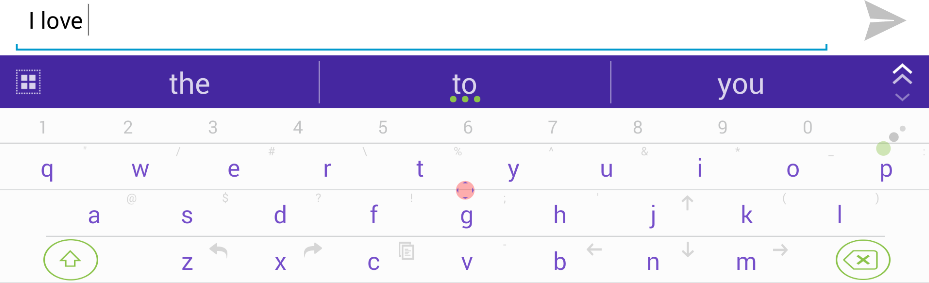
\includegraphics[width=0.9\textwidth]{figures/smartphone}}

    \vspace{0.6cm}

    \LARGE
    Guess the \emph{next intended} word
    \\[0.2cm]
    from words already entered
  \end{center}
\end{frame}


\begin{frame}
  \frametitle{Benefits of good Word Prediction}

  \large
  \begin{itemize}
    \item Faster typing
    \vspace{0.5cm}
    \item Spelling / Grammar
    \vspace{0.5cm}
    \item \ldots
    \vspace{0.5cm}
    \item Metric for Language Models?
  \end{itemize}
\end{frame}

\begin{frame}[t]
  \frametitle{Thesis Goal}

  \begin{center}
    \Large
    Word prediction usually optimized for\\speed \textbf{or} quality

    \vspace{3.3cm}

    \onslide<2->{
      This thesis optimizes for speed while\\maintaining best quality!
    }

    \vspace{-4.1cm}
    \begin{tikzpicture}[
      remember picture,
      overlay,
    ]
      \draw [<->, thick]
        (-4.5,0cm) node [below, align = center, yshift = -0.25cm] {Calculation\\Time}
        --
        ( 4.5,0cm) node [below, align = center, yshift = -0.25cm] {Prediction\\Quality};

      \draw [thick]
        (0,0.2cm) -- (0,-0.2cm) node [below, align = center, yshift = -0.15cm] {\LARGE\textbf{?}\\[-1ex]\large$\longleftrightarrow$};
    \end{tikzpicture}
  \end{center}
\end{frame}

\begin{frame}
  \frametitle{Next Word Prediction}

  \LARGE
  \begin{equation*}
    \only<1-3>{\phantom{_{p}}\NWP{\tikzmark{hist1_fst}h} = \Argmax{\mathclap{\substack{w \in \Vocab\\\phantom{p \: \text{prefix of} \: w}}}}\tikzmark{vocab_fst} \Prob{\tikzmark{w_fst}w}{\tikzmark{hist2_fst}h}}
    %\only<4- >{\NWP[\tikzmark{prefix}p]{\tikzmark{hist1_snd}h} = \Argmax{\mathclap{\substack{w \in \Vocab,\\p \: \text{prefix of} \: w}}}\tikzmark{vocab_snd} \Prob{\tikzmark{w_snd}w}{\tikzmark{hist2_snd}h}}
  \end{equation*}

  \large
  
\begin{tikzpicture}[
    remember picture,
    overlay,
    expl/.style = {draw = Maroon, rounded corners, thick},
    arrow/.style = {Maroon, thick, ->, >=latex},
  ]
    \node<2->[expl]
      (hist_expl) at (2,3.5cm) {history of entered words};
    \node<3->[expl]
      (vocab_expl) at (8.5,-1.5cm) {for each word in vocabulary};
%     \node<4->[expl, align=center]
%       (prefix_expl) at (2.5,-1cm) {entered prefix of\\intended word};
    \LARGE % restore equation size so font relative units are correct
    \draw<2-3>[arrow] (hist_expl.south)   to [out=270, in=100] ([xshift= 0.2em, yshift= 2.0ex]{pic cs:hist1_fst});
    \draw<2-3>[arrow] (hist_expl.east)    to [out=  0, in=100] ([xshift= 0.2em, yshift= 2.0ex]{pic cs:hist2_fst});
%     \draw<4- >[arrow] (hist_expl.south)   to [out=270, in=100] ([xshift= 0.2em, yshift= 2.0ex]{pic cs:hist1_snd});
%     \draw<4- >[arrow] (hist_expl.east)    to [out=  0, in=100] ([xshift= 0.2em, yshift= 2.0ex]{pic cs:hist2_snd});
    \draw<3  >[arrow] (vocab_expl.north)  to [out= 90, in=  0] ([xshift=-0.7em, yshift=-1.3ex]{pic cs:vocab_fst});
    \draw<3  >[arrow] (vocab_expl.north)  to [out= 90, in=270] ([xshift= 0.4em, yshift=-0.6ex]{pic cs:w_fst});
%     \draw<4- >[arrow] (vocab_expl.north)  to [out= 90, in=  0] ([xshift=-0.7em, yshift=-1.3ex]{pic cs:vocab_snd});
%     \draw<4- >[arrow] (vocab_expl.north)  to [out= 90, in=270] ([xshift= 0.4em, yshift=-0.6ex]{pic cs:w_snd});
%     \draw<4- >[arrow] (prefix_expl.north) to [out= 90, in=270] ([xshift= 0.2em, yshift=-0.9ex]{pic cs:prefix});
%     \draw<4- >[arrow] (prefix_expl.north) to [out= 90, in=180] ([xshift=-5.2em, yshift=-3.0ex]{pic cs:w_snd});
  \end{tikzpicture}
\end{frame}


% ==============================================================================
\section{Language Models}
\subsection{}

\begin{frame}
  \frametitle{How to find probabilities?}

  \begin{center}
    \LARGE $\Prob{w}{h}$ ?
  \end{center}

  \vspace{0.5cm}

  \onslide<2->{
    \large
    Solution: Statistical Language Models
    \begin{itemize}
      \item analyze text corpora
      \item to estimate sequence probabilities
    \end{itemize}
  }

  \vspace{0.5cm}

  \onslide<3->{
    \large
    We will employ two state-of-the-art Language Models:
    \begin{itemize}
      \item Modified Kneser Ney Smoothing\\[-0.4ex]{\small\parencite{ChenGoodman1999}}
      \item Generalized Language Model\\[-0.4ex]{\small\parencite{Pickhardt2014}}
    \end{itemize}
  }
\end{frame}

\begin{frame}
  \frametitle{Modified Kneser Ney Smoothing}

  \only<1-2>{
    \large
    \begin{align*}
      \ProbMKN{w_n}{w_1^{n-1}} &=
        \frac{\DiscountedCount(w_1^n) + \gamma(w_1^{n-1}) \tikzmark{recmkn_high}\ProbMKN*{w_n}{w_2^{n-1}}}
             {\Count(w_1^{n-1} \Skp)} \\
      %\intertext{\vspace{0.4cm}}
      %\ProbMKN*{w_n}{w_1^{n-1}} &=
      %  \frac{\DiscountedCount*(\WSkp w_1^n) + \gamma(w_1^{n-1}) \tikzmark{recmkn_low}\ProbMKN*{w_n}{w_2^{n-1}}}
      %     {\ContCountIp(\WSkp w_1^{n-1} \WSkp)}
    \end{align*}

    
\begin{tikzpicture}[
      remember picture,
      overlay,
    ]
      \draw<2>[Maroon, ultra thick] (pic cs:recmkn_high) ellipse
        [xshift=4em, yshift=0.6ex, x radius=4.5em, y radius=3ex];
      %\draw<2>[Maroon, ultra thick] (pic cs:recmkn_low)  ellipse
      %  [xshift=4em, yshift=0.6ex, x radius=4.5em, y radius=3ex];
    \end{tikzpicture}
  }

  %\only<3>{
  %  \begin{center}
  %    \begin{tikzpicture}
  %      \tikzset{
  %        every node/.style = {scale = 0.7},
  %        state/.style  = {draw, circle, align = center, text centered, text width = 4.2em},
  %        invis/.style  = {text width = 4.2em},
  %        order/.style  = {align = center, text centered, text width = 4em, text = Maroon},
  %      }
  %
  %      \begin{scope}[node distance = 7em]
  %        \node [state] (highest)                    {$w_1 \: w_2 \: w_3$};
  %        \node [state] (lower1)  [below of=highest] {$w_2 \: w_3$};
  %        \node [state] (lower2)  [below of=lower1]  {$w_3$};
  %        \node [state] (lowest)  [below of=lower2]  {$\EmptyNGram$};
  %      \end{scope}
  %
  %      \begin{scope}[node distance = 5.5em]
  %        \node [order] [right of=highest] {$\ProbMKN {w_4}{w_1 w_2 w_3}$};
  %        \node [order] [right of=lower1]  {$\ProbMKN*{w_4}{w_2 w_3}$};
  %        \node [order] [right of=lower2]  {$\ProbMKN*{w_4}{w_3}$};
  %        \node [order] [right of=lowest]  {$\ProbMKN*{w_4}$};
  %      \end{scope}
  %
  %      \path[->, >=latex, thick]
  %        (highest) edge (lower1)
  %        (lower1)  edge (lower2)
  %        (lower2)  edge (lowest);
  %    \end{tikzpicture}
  %  \end{center}
  %}
\end{frame}

\begin{frame}
  \frametitle{Generalized Language Model}

  \only<1-2>{
    \begin{align*}
      \hspace{-1.5em}
      \ProbGLM{w_n}{w_1^{n-1}} &=
        \frac{\DiscountedCount(w_1^n) + \frac{\gamma(w_1^{n-1})}{\NumSkpOp{w_1^{n-1}}}
                                        \tikzmark{recglm_high}\sum_{j=1}^{\NumSkpOp{w_1^{n-1}}} \ProbGLM*{w_n}{\SkpOp[j]{w_1^{n-1}}}}
            {\Count(w_1^{n-1} \Skp)} \\
      %\intertext{\vspace{0.4cm}}
      %\hspace{-1.5em}
      %\ProbGLM*{w_n}{w_1^{n-1}} &=
      %\frac{\DiscountedCount*(\WSkp w_1^n) + \frac{\gamma(w_1^{n-1})}{\NumSkpOp{w_1^{n-1}}}
      %                                        \tikzmark{recglm_low}\sum_{j=1}^{\NumSkpOp{w_1^{n-1}}} \ProbGLM*{w_n}{\SkpOp[j]{w_1^{n-1}}}}
      %    {\ContCountIp(\WSkp w_1^{n-1} \WSkp)}
    \end{align*}

    
\begin{tikzpicture}[
      remember picture,
      overlay,
    ]
      \draw<2>[Maroon, ultra thick] (pic cs:recglm_high) ellipse
        [xshift=6.7em, yshift=0.6ex, x radius=7.2em, y radius=4ex];
      %\draw<2>[Maroon, ultra thick] (pic cs:recglm_low)  ellipse
      %  [xshift=6.7em, yshift=0.6ex, x radius=7.2em, y radius=4ex];
      \end{tikzpicture}
  }

  %\only<3>{
  %  \begin{center}
  %    \begin{tikzpicture}
  %      \tikzset{
  %        every node/.style = {scale = 0.8},
  %        state/.style  = {draw, circle, align = center, text centered, text width = 4.2em},
  %        invis/.style  = {text width = 4.2em},
  %        order/.style  = {align = center, text centered, text width = 4em, text = Maroon},
  %      }
  %
  %      \begin{scope}[node distance = 6.5em]
  %        \node [state] (000)                  {$w_1 \: w_2 \: w_3$};
  %        \node [invis] (000l) [left  of=000]  {};
  %        \node [invis] (000r) [right of=000]  {};
  %
  %        \node [state] (001)  [below of=000l] {$w_1 \: w_2 \: \Skp$};
  %        \node [state] (010)  [below of=000]  {$w_1 \: \Skp \: w_3$};
  %        \node [state] (100)  [below of=000r] {$\Skp \: w_2 \: w_3$};
  %
  %        \node [state] (011)  [below of=001] {$w_1 \: \Skp \: \Skp$};
  %        \node [state] (101)  [below of=010] {$\Skp \: w_2 \: \Skp$};
  %        \node [state] (110)  [below of=100] {$\Skp \: \Skp \: w_3$};
  %
  %        \node [state] (111)  [below of=101] {$\Skp \: \Skp \: \Skp$};
  %        \node [invis] (111l) [below of=011] {};
  %        \node [invis] (111r) [below of=110] {};
  %      \end{scope}
  %
  %      \begin{scope}[node distance = 5.5em]
  %        \node [order] [right of=000] {$\ProbGLM {w_4}{w_1 w_2 w_3}$};
  %      \end{scope}
  %
  %      \path[->, >=latex, thick]
  %        (000) edge (001)
  %        (000) edge (010)
  %        (000) edge (100)
  %
  %        (001) edge (011)
  %        (001) edge (101)
  %        (010) edge (011)
  %        (010) edge (110)
  %        (100) edge (101)
  %        (100) edge (110)
  %
  %        (011) edge (111)
  %        (101) edge (111)
  %        (110) edge (111);
  %    \end{tikzpicture}
  %  \end{center}
  %}
\end{frame}

\iffalse
\begin{frame}
  \frametitle{Backoff Graph}

  \begin{textblock}{10}(4.4,-0.9)
    \raggedleft
    \only<1>{Modified Kneser Ney Smoothing}
    \only<2>{Generalized Language Model}
  \end{textblock}

  \vspace{-0.7cm}
  \begin{center}
    \begin{tikzpicture}
      \tikzset{
        every node/.style = {scale = 0.8},
        state/.style  = {draw, circle, align = center, text centered, text width = 4.2em},
        invis/.style  = {text width = 4.2em},
        order/.style  = {align = center, text centered, text width = 4em, text = Maroon},
      }

      \only<1>{
        \begin{scope}[node distance = 7em]
          \node [state] (highest)                    {$w_1 \: w_2 \: w_3$};
          \node [state] (lower1)  [below of=highest] {$w_2 \: w_3$};
          \node [state] (lower2)  [below of=lower1]  {$w_3$};
          \node [state] (lowest)  [below of=lower2]  {$\EmptyNGram$};
        \end{scope}

        \begin{scope}[node distance = 5.5em]
          \node [order] [right of=highest] {$\ProbMKN {w_4}{w_1 w_2 w_3}$};
          \node [order] [right of=lower1]  {$\ProbMKN*{w_4}{w_2 w_3}$};
          \node [order] [right of=lower2]  {$\ProbMKN*{w_4}{w_3}$};
          \node [order] [right of=lowest]  {$\ProbMKN*{w_4}$};
        \end{scope}

        \path[->, >=latex, thick]
          (highest) edge (lower1)
          (lower1)  edge (lower2)
          (lower2)  edge (lowest);
      }

      \only<2>{
        \begin{scope}[node distance = 6.5em]
          \node [state] (000)                  {$w_1 \: w_2 \: w_3$};
          \node [invis] (000l) [left  of=000]  {};
          \node [invis] (000r) [right of=000]  {};

          \node [state] (001)  [below of=000l] {$w_1 \: w_2 \: \Skp$};
          \node [state] (010)  [below of=000]  {$w_1 \: \Skp \: w_3$};
          \node [state] (100)  [below of=000r] {$\Skp \: w_2 \: w_3$};

          \node [state] (011)  [below of=001] {$w_1 \: \Skp \: \Skp$};
          \node [state] (101)  [below of=010] {$\Skp \: w_2 \: \Skp$};
          \node [state] (110)  [below of=100] {$\Skp \: \Skp \: w_3$};

          \node [state] (111)  [below of=101] {$\Skp \: \Skp \: \Skp$};
          \node [invis] (111l) [below of=011] {};
          \node [invis] (111r) [below of=110] {};
        \end{scope}

        \path[->, >=latex, thick]
          (000) edge (001)
          (000) edge (010)
          (000) edge (100)

          (001) edge (011)
          (001) edge (101)
          (010) edge (011)
          (010) edge (110)
          (100) edge (101)
          (100) edge (110)

          (011) edge (111)
          (101) edge (111)
          (110) edge (111);
      }
    \end{tikzpicture}
  \end{center}
\end{frame}
\fi

\newcommand{\ProbMKNcab}[1]
  {\frac{\tikzmark{you_1}\DiscountedCount(\text{I love you}) + \gamma(\text{I love}) #1}{\Count(\text{I love\Skp})}}
\newcommand{\ProbMKNcb}[1]
  {\frac{\tikzmark{you_2}\DiscountedCount*(\text{\WSkp love you}) + \gamma(\text{love}) #1}{\ContCountIp(\text{\WSkp love \WSkp})}}
\newcommand{\ProbMKNc}
  {\frac{\tikzmark{you_3}\ContCountIp(\text{\WSkp you})}{\ContCountIp(\text{\WSkp \WSkp})}}

\begin{frame}
  \frametitle{Example: Probability of \enquote{you} after \enquote{I love}}

  \large
  \begin{align*}
    \hspace{-0.5cm}
    \ProbMKN {\text{you}}{\text{I love}} &= \ProbMKNcab{\ProbMKN*{\text{you}}{\text{love}}} \\
    \intertext{\vspace{0.2cm}}
    \hspace{-0.5cm}
    \ProbMKN*{\text{you}}{\text{love}}   &= \ProbMKNcb{\ProbMKN*{\text{you}}} \\
    \intertext{\vspace{0.2cm}}
    \hspace{-0.5cm}
    \ProbMKN*{\text{you}}                &= \ProbMKNc
  \end{align*}

  
\begin{tikzpicture}[
    remember picture,
    overlay,
  ]
    \draw<2->[Maroon, ultra thick] (pic cs:you_1) ellipse
      [xshift=3.2em, yshift=0.6ex, x radius=3.6em, y radius=3ex];
    \draw<2->[Maroon, ultra thick] (pic cs:you_2)  ellipse
      [xshift=3.3em, yshift=0.6ex, x radius=3.8em, y radius=3ex];
    \draw<2->[Maroon, ultra thick] (pic cs:you_3)  ellipse
      [xshift=2.6em, yshift=0.6ex, x radius=2.8em, y radius=3ex];
  \end{tikzpicture}
\end{frame}

\begin{frame}
  \frametitle{Idea: express as Weighted Sums}

  \LARGE
  \begin{equation*}
    \Prob{\tikzmark{argw}w}{\tikzmark{argh}h} = \sum_{i = 1}^{N} \tikzmark{sumweight}\SumWeight_i^h \; \tikzmark{sumarg}\SumArg_i^h(w)
  \end{equation*}

  \large
  \begin{tikzpicture}[
    remember picture,
    overlay,
    expl/.style = {draw = Maroon, rounded corners, thick},
    arrow/.style = {Maroon, thick, ->, >=latex},
  ]
    \node<2->[expl]
      (sumarg_expl) at (7.6,4.0cm) {depends on argument $w$};
    \node<3->[expl]
      (sumweight_expl) at (2.5,3.0cm) {independent of argument $w$};
    \node<4->[expl]
      (argw_expl) at (3.2,-1.7cm) {all words in vocabulary};
    \node<5->[expl]
      (argh_expl) at (7.2,-0.7cm) {user given, thus fixed};
    \LARGE % restore equation size so font relative units are correct
    \draw<2->[arrow] (sumarg_expl.south)   to [out=270, in= 90] ([xshift= 1.1em, yshift= 2.2ex]{pic cs:sumarg});
    \draw<3->[arrow] (sumweight_expl.east) to [out=  0, in= 90] ([xshift= 0.4em, yshift= 2.2ex]{pic cs:sumweight});
    \draw<4->[arrow] (argw_expl.north)     to [out= 90, in=270] ([xshift= 0.4em, yshift=-0.9ex]{pic cs:argw});
    \draw<5->[arrow] (argh_expl.west)      to [out=180, in=270] ([xshift= 0.4em, yshift=-0.9ex]{pic cs:argh});
  \end{tikzpicture}
\end{frame}

\begin{frame}[plain]
  \centering
  \begin{minipage}{0.9\textwidth}
    \centering
    \only<1>{
      \documentclass{standalone}
\usepackage[dvipsnames,svgnames,x11names]{xcolor}
\usepackage{tikz}
\usepackage{pgfplots}
\usetikzlibrary{pgfplots.statistics}
\pgfplotsset{compat = 1.12}
\usepackage[
  group-separator={,},
  exponent-product=\cdot,
  binary-units = true,
]{siunitx}
\usepackage{../thesismath}
\begin{document}
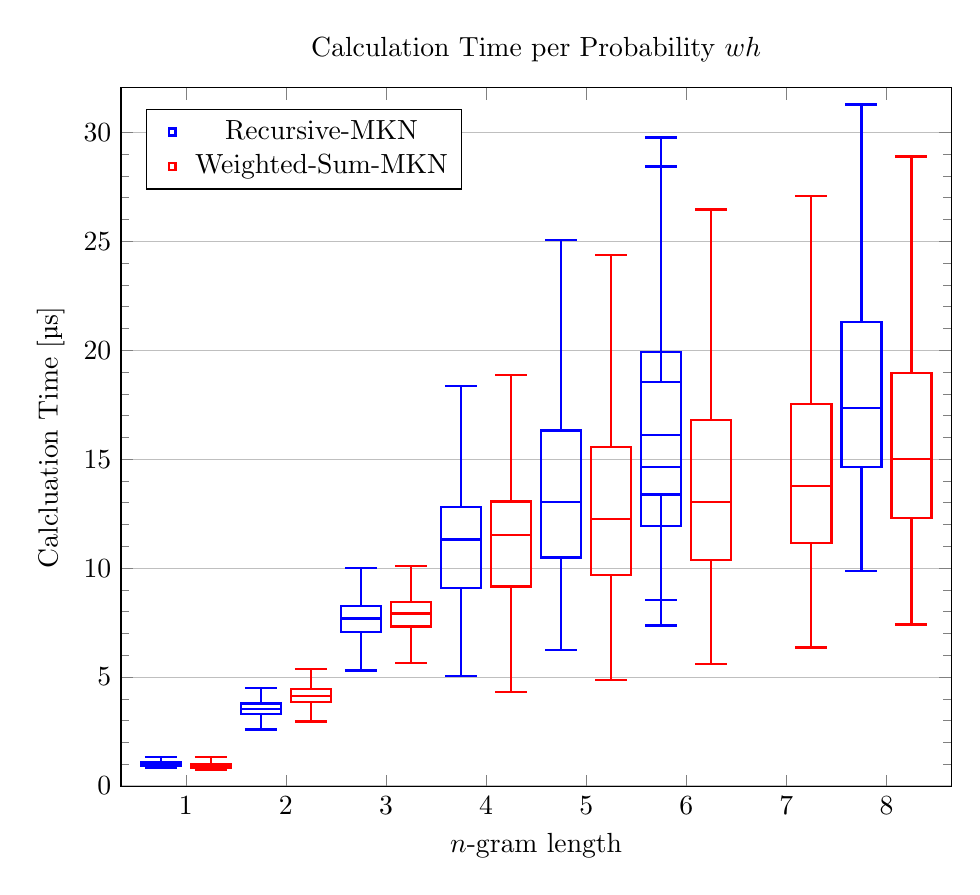
\begin{tikzpicture}[baseline]

\pgfplotscreateplotcyclelist{recmkn_mkn}{%
  blue,  mark size=1.25, mark=square, thick,\\%
  red,   mark size=1.25, mark=square, thick,\\%
}

\pgfplotsset{
  legend style = {
    legend image code/.code = {
      \draw[only marks]
        plot coordinates {
          (0.3cm,0cm)
        };
      \node at (0.15cm, 0cm) {};
      \node at (0.45cm, 0cm) {};
    },
  },
  boxplot/draw/average/.code = {
    %\draw[dashed, /pgfplots/boxplot/every average/.try]
    %  (boxplot box cs:\pgfplotsboxplotvalue{average},0)
    %  --
    %  (boxplot box cs:\pgfplotsboxplotvalue{average},1)
    %  ;
  },
}

\begin{axis}[
  title = {Calculation Time per Probability $\ProbMKN{w}{h}$},
  xlabel = {$n$-gram length},
  xtick = {1, ..., 8},
  ylabel = {Calcluation Time [\si{\micro\second}]},
  minor y tick num = 4,
  log ticks with fixed point,
  ymajorgrids = true,
  boxplot/draw direction = y,
  boxplot = {
    draw position = {3/4 + floor(\plotnumofactualtype/2) + 2/4*mod(\plotnumofactualtype,2)},
    box extend = 0.4,
  },
  cycle list name = recmkn_mkn,
  enlargelimits = 0.025,
  legend entries = {{Recursive-MKN}, {Weighted-Sum-MKN}},
  legend pos = north west,
  width = \textwidth,
]

% ------------------------------------------------------------------------------

% ngram-1-Fast-Modified-Kneser-Ney
\addplot+[
  boxplot prepared = {
    lower whisker = 0.830,
    lower quartile = 0.940,
    median = 0.993,
    upper quartile = 1.090,
    upper whisker = 1.315,
    average = 1.076,
  },
] table [row sep = \\, y index = 0] {
  data\\
};

% ngram-1-Weighted-Sum-Modified-Kneser-Ney
\addplot+[
  boxplot prepared = {
    lower whisker = 0.726,
    lower quartile = 0.825,
    median = 0.908,
    upper quartile = 1.025,
    upper whisker = 1.325,
    average = 1.011,
  },
] table [row sep = \\, y index = 0] {
  data\\
};

% ------------------------------------------------------------------------------

% ngram-2-Fast-Modified-Kneser-Ney
\addplot+[
  boxplot prepared = {
    lower whisker = 2.591,
    lower quartile = 3.309,
    median = 3.542,
    upper quartile = 3.789,
    upper whisker = 4.509,
    average = 3.731,
  },
] table [row sep = \\, y index = 0] {
  data\\
};

% ngram-2-Weighted-Sum-Modified-Kneser-Ney
\addplot+[
  boxplot prepared = {
    lower whisker = 2.964,
    lower quartile = 3.854,
    median = 4.146,
    upper quartile = 4.454,
    upper whisker = 5.354,
    average = 4.306,
  },
] table [row sep = \\, y index = 0] {
  data\\
};

% ------------------------------------------------------------------------------

% ngram-3-Fast-Modified-Kneser-Ney
\addplot+[
  boxplot prepared = {
    lower whisker = 5.303,
    lower quartile = 7.070,
    median = 7.692,
    upper quartile = 8.248,
    upper whisker = 10.012,
    average = 7.731,
  },
] table [row sep = \\, y index = 0] {
  data\\
};

% ngram-3-Weighted-Sum-Modified-Kneser-Ney
\addplot+[
  boxplot prepared = {
    lower whisker = 5.653,
    lower quartile = 7.319,
    median = 7.921,
    upper quartile = 8.430,
    upper whisker = 10.089,
    average = 8.081,
  },
] table [row sep = \\, y index = 0] {
  data\\
};

% ------------------------------------------------------------------------------

% ngram-4-Fast-Modified-Kneser-Ney
\addplot+[
  boxplot prepared = {
    lower whisker = 5.036,
    lower quartile = 9.101,
    median = 11.313,
    upper quartile = 12.809,
    upper whisker = 18.367,
    average = 11.068,
  },
] table [row sep = \\, y index = 0] {
  data\\
};

% ngram-4-Weighted-Sum-Modified-Kneser-Ney
\addplot+[
  boxplot prepared = {
    lower whisker = 4.297,
    lower quartile = 9.160,
    median = 11.517,
    upper quartile = 13.053,
    upper whisker = 18.88,
    average = 11.374,
  },
] table [row sep = \\, y index = 0] {
  data\\
};

% ------------------------------------------------------------------------------

% ngram-5-Fast-Modified-Kneser-Ney
\addplot+[
  boxplot prepared = {
    lower whisker = 6.252,
    lower quartile = 10.484,
    median = 13.016,
    upper quartile = 16.311,
    upper whisker = 25.042,
    average = 13.591,
  },
] table [row sep = \\, y index = 0] {
  data\\
};

% ngram-5-Weighted-Sum-Modified-Kneser-Ney
\addplot+[
  boxplot prepared = {
    lower whisker = 4.852,
    lower quartile = 9.669,
    median = 12.238,
    upper quartile = 15.555,
    upper whisker = 24.382,
    average = 12.666,
  },
] table [row sep = \\, y index = 0] {
  data\\
};


% ------------------------------------------------------------------------------

% ngram-6-Fast-Modified-Kneser-Ney
\addplot+[
  boxplot prepared = {
    lower whisker = 7.367,
    lower quartile = 11.917,
    median = 14.650,
    upper quartile = 18.526,
    upper whisker = 28.432,
    average = 15.903,
  },
] table [row sep = \\, y index = 0] {
  data\\
};

% ngram-6-Weighted-Sum-Modified-Kneser-Ney
\addplot+[
  boxplot prepared = {
    lower whisker = 5.609,
    lower quartile = 10.380,
    median = 13.040,
    upper quartile = 16.812,
    upper whisker = 26.460,
    average = 14.117,
  },
] table [row sep = \\, y index = 0] {
  data\\
};


% ------------------------------------------------------------------------------

% ngram-7-Fast-Modified-Kneser-Ney
\addplot+[
  boxplot prepared = {
    lower whisker = 8.519,
    lower quartile = 13.383,
    median = 16.117,
    upper quartile = 19.934,
    upper whisker = 29.760,
    average = 17.739,
  },
] table [row sep = \\, y index = 0] {
  data\\
};

% ngram-7-Weighted-Sum-Modified-Kneser-Ney
\addplot+[
  boxplot prepared = {
    lower whisker = 6.352,
    lower quartile = 11.159,
    median = 13.782,
    upper quartile = 17.521,
    upper whisker = 27.062,
    average = 15.302,
  },
] table [row sep = \\, y index = 0] {
  data\\
};


% ------------------------------------------------------------------------------

% ngram-8-Fast-Modified-Kneser-Ney
\addplot+[
  boxplot prepared = {
    lower whisker = 9.868,
    lower quartile = 14.658,
    median = 17.365,
    upper quartile = 21.310,
    upper whisker = 31.276,
    average = 19.446,
  },
] table [row sep = \\, y index = 0] {
  data\\
};

% ngram-8-Weighted-Sum-Modified-Kneser-Ney
\addplot+[
  boxplot prepared = {
    lower whisker = 7.413,
    lower quartile = 12.307,
    median = 15.013,
    upper quartile = 18.940,
    upper whisker = 28.889,
    average = 16.963,
  },
] table [row sep = \\, y index = 0] {
  data\\
};

\end{axis}

\end{tikzpicture}
\end{document}
}
    \only<2>{
      \documentclass{standalone}
\usepackage[dvipsnames,svgnames,x11names]{xcolor}
\usepackage{tikz}
\usepackage{pgfplots}
\usetikzlibrary{pgfplots.statistics}
\pgfplotsset{compat = 1.12}
\usepackage[
  group-separator={,},
  exponent-product=\cdot,
  binary-units = true,
]{siunitx}
\usepackage{../thesismath}
\begin{document}
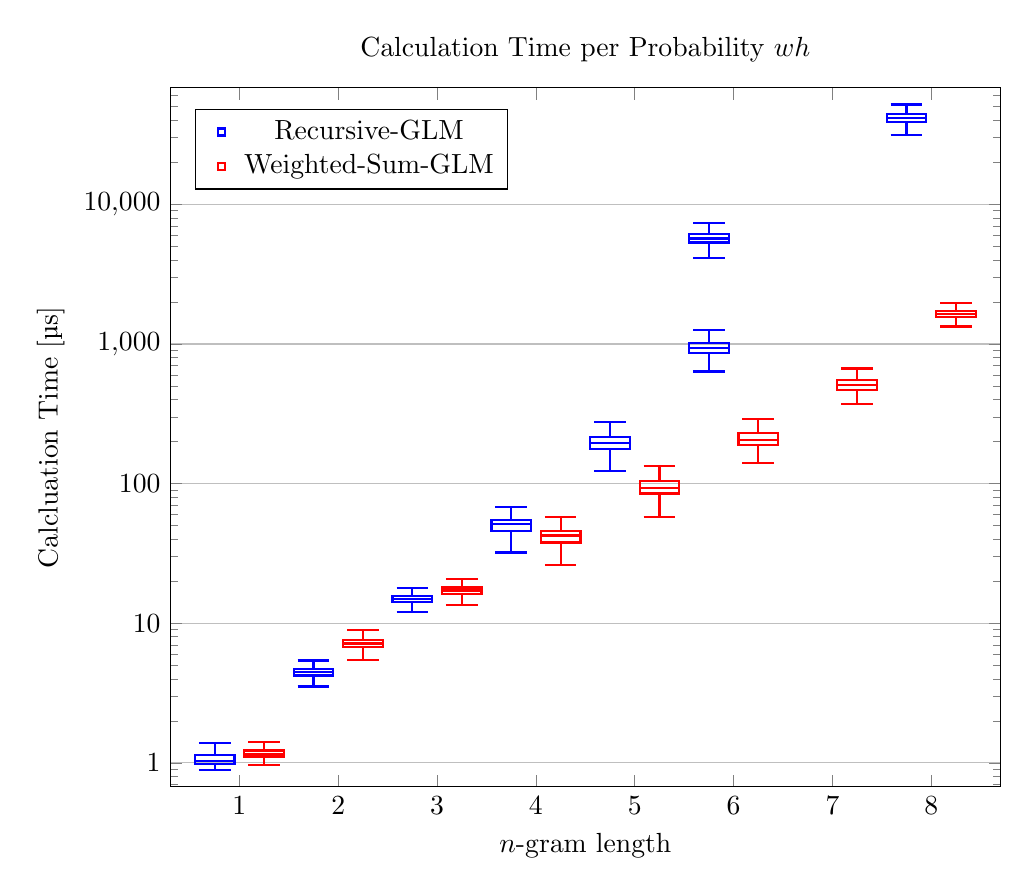
\begin{tikzpicture}[baseline]

\pgfplotscreateplotcyclelist{recglm_glm}{%
  blue,  mark size=1.25, mark=square, thick,\\%
  red,   mark size=1.25, mark=square, thick,\\%
}

\pgfplotsset{
  legend style = {
    legend image code/.code = {
      \draw[only marks]
        plot coordinates {
          (0.3cm,0cm)
        };
      \node at (0.15cm, 0cm) {};
      \node at (0.45cm, 0cm) {};
    },
  },
  boxplot/draw/average/.code = {
    %\draw[dashed, /pgfplots/boxplot/every average/.try]
    %  (boxplot box cs:\pgfplotsboxplotvalue{average},0)
    %  --
    %  (boxplot box cs:\pgfplotsboxplotvalue{average},1)
    %  ;
  },
}

\begin{axis}[
  title = {Calculation Time per Probability $\ProbGLM{w}{h}$},
  xlabel = {$n$-gram length},
  xtick = {1, ..., 8},
  xmin = 0.5,
  xmax = 8.5,
  ylabel = {Calcluation Time [\si{\micro\second}]},
  ymax = 0.886,
  ymax = 51890.229,
  ymode = log,
  log ticks with fixed point,
  ymajorgrids = true,
  boxplot/draw direction = y,
  boxplot = {
    draw position = {3/4 + floor(\plotnumofactualtype/2) + 2/4*mod(\plotnumofactualtype,2)},
    box extend = 0.4,
  },
  cycle list name = recglm_glm,
  enlargelimits = 0.025,
  legend entries = {{Recursive-GLM}, {Weighted-Sum-GLM}},
  legend pos = north west,
  width = \textwidth,
]

% ------------------------------------------------------------------------------

% ngram-1-Fast-Generalized-Language-Model
\addplot+[
  boxplot prepared = {
    lower whisker = 0.886,
    lower quartile = 0.977,
    median = 1.030,
    upper quartile = 1.138,
    upper whisker = 1.379,
    average = 1.158,
  },
] table [row sep = \\, y index = 0] {
  data\\
};

% ngram-1-Weighted-Sum-Generalized-Language-Model
\addplot+[
  boxplot prepared = {
    lower whisker = 0.967,
    lower quartile = 1.098,
    median = 1.146,
    upper quartile = 1.226,
    upper whisker = 1.418,
    average = 1.207,
  },
] table [row sep = \\, y index = 0] {
  data\\
};

% ------------------------------------------------------------------------------

% ngram-2-Fast-Generalized-Language-Model
\addplot+[
  boxplot prepared = {
    lower whisker = 3.528,
    lower quartile = 4.230,
    median = 4.463,
    upper quartile = 4.705,
    upper whisker = 5.416,
    average = 4.596,
  },
] table [row sep = \\, y index = 0] {
  data\\
};

% ngram-2-Weighted-Sum-Generalized-Language-Model
\addplot+[
  boxplot prepared = {
    lower whisker = 5.432,
    lower quartile = 6.742,
    median = 7.159,
    upper quartile = 7.629,
    upper whisker = 8.954,
    average = 7.475,
  },
] table [row sep = \\, y index = 0] {
  data\\
};

% ------------------------------------------------------------------------------

% ngram-3-Fast-Generalized-Language-Model
\addplot+[
  boxplot prepared = {
    lower whisker = 11.990,
    lower quartile = 14.202,
    median = 14.974,
    upper quartile = 15.677,
    upper whisker = 17.887,
    average = 15.200,
  },
] table [row sep = \\, y index = 0] {
  data\\
};

% ngram-3-Weighted-Sum-Generalized-Language-Model
\addplot+[
  boxplot prepared = {
    lower whisker = 13.591,
    lower quartile = 16.268,
    median = 17.176,
    upper quartile = 18.053,
    upper whisker = 20.728,
    average = 17.503,
  },
] table [row sep = \\, y index = 0] {
  data\\
};

% ------------------------------------------------------------------------------

% ngram-4-Fast-Generalized-Language-Model
\addplot+[
  boxplot prepared = {
    lower whisker = 32.142,
    lower quartile = 45.684,
    median = 51.305,
    upper quartile = 54.749,
    upper whisker = 68.338,
    average = 51.656,
  },
] table [row sep = \\, y index = 0] {
  data\\
};

% ngram-4-Weighted-Sum-Generalized-Language-Model
\addplot+[
  boxplot prepared = {
    lower whisker = 26.132,
    lower quartile = 37.833,
    median = 42.526,
    upper quartile = 45.800,
    upper whisker = 57.742,
    average = 43.166,
  },
] table [row sep = \\, y index = 0] {
  data\\
};

% ------------------------------------------------------------------------------

% ngram-5-Fast-Generalized-Language-Model
\addplot+[
  boxplot prepared = {
    lower whisker = 123.586,
    lower quartile = 176.243,
    median = 194.149,
    upper quartile = 215.771,
    upper whisker = 274.831,
    average = 208.875,
  },
] table [row sep = \\, y index = 0] {
  data\\
};

% ngram-5-Weighted-Sum-Generalized-Language-Model
\addplot+[
  boxplot prepared = {
    lower whisker = 57.479,
    lower quartile = 85.049,
    median = 93.283,
    upper quartile = 104.396,
    upper whisker = 133.392,
    average = 95.882,
  },
] table [row sep = \\, y index = 0] {
  data\\
};

% ------------------------------------------------------------------------------

% ngram-6-Fast-Generalized-Language-Model
\addplot+[
  boxplot prepared = {
    lower whisker = 634.356,
    lower quartile = 864.441,
    median = 935.081,
    upper quartile = 1022.439,
    upper whisker = 1259.275,
    average = 1085.126,
  },
] table [row sep = \\, y index = 0] {
  data\\
};

% ngram-6-Weighted-Sum-Generalized-Language-Model
\addplot+[
  boxplot prepared = {
    lower whisker = 140.713,
    lower quartile = 188.745,
    median = 206.247,
    upper quartile = 230.087,
    upper whisker = 292.096,
    average = 214.342,
  },
] table [row sep = \\, y index = 0] {
  data\\
};

% ------------------------------------------------------------------------------

% ngram-7-Fast-Generalized-Language-Model
\addplot+[
  boxplot prepared = {
    lower whisker = 4144.340,
    lower quartile = 5337.246,
    median = 5703.376,
    upper quartile = 6141.529,
    upper whisker = 7346.732,
    average = 5814.210,
  },
] table [row sep = \\, y index = 0] {
  data\\
};

% ngram-7-Weighted-Sum-Generalized-Language-Model
\addplot+[
  boxplot prepared = {
    lower whisker = 371.056,
    lower quartile = 470.873,
    median = 505.111,
    upper quartile = 549.414,
    upper whisker = 667.226,
    average = 538.550,
  },
] table [row sep = \\, y index = 0] {
  data\\
};

% ------------------------------------------------------------------------------

% ngram-8-Fast-Generalized-Language-Model
\addplot+[
  boxplot prepared = {
    lower whisker = 31374.542,
    lower quartile = 39013.754,
    median = 41361.691,
    upper quartile = 44166.572,
    upper whisker = 51890.229,
    average = 42025.650,
  },
] table [row sep = \\, y index = 0] {
  data\\
};

% ngram-8-Weighted-Sum-Generalized-Language-Model
\addplot+[
  boxplot prepared = {
    lower whisker = 1334.356,
    lower quartile = 1565.650,
    median = 1637.919,
    upper quartile = 1720.993,
    upper whisker = 1953.776,
    average = 1652.884,
  },
] table [row sep = \\, y index = 0] {
  data\\
};

\end{axis}

% \begin{axis}[
% % http://www.latex-community.org/forum/viewtopic.php?f=45&p=71073
% %       xmin = 750, xmax = 2000,
% %       ymin = 1400, ymax = 1800,
%   hide x axis,
%   axis y line*=right,
% %       ylabel={$T_e$ (\si{\fahrenheit})},
% %       ylabel near ticks
%   width = \textwidth,
% ]
% \end{axis}


\end{tikzpicture}
\end{document}
}
  \end{minipage}
\end{frame}

\begin{frame}[plain]
  \centering
  \begin{minipage}{0.9\textwidth}
    \includestandalone{figures/presentation-weight-times}
  \end{minipage}
\end{frame}


% ==============================================================================
\section{Top-k Joining Techniques}
\subsection{}

\begin{frame}
  \frametitle{What are Top-k Join Queries?}

  \begin{center}
    \onslide<2->{
      \fbox{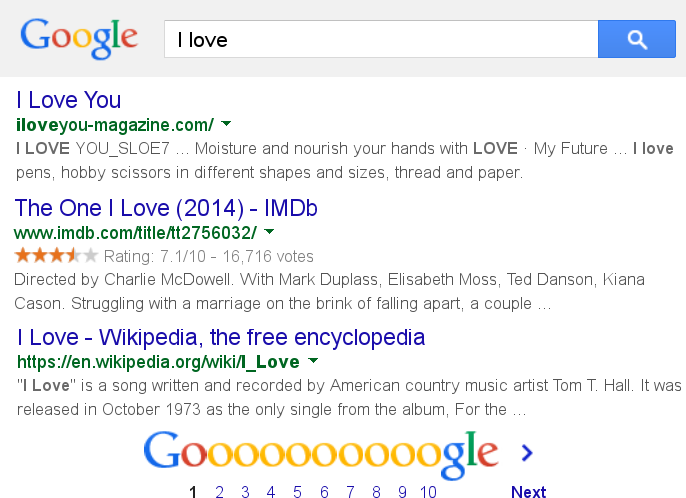
\includegraphics[width=0.8\textwidth]{figures/google-results}}}
  \end{center}

  \large
  \begin{tikzpicture}[
    remember picture,
    overlay,
    expl/.style = {draw = Maroon, rounded corners, thick, fill=white},
    arrow/.style = {Maroon, thick, ->, >=latex},
  ]
    \node<3->[expl, align=left, anchor=north] at (9cm, 7.5cm) {
      \begin{varwidth}{4.1cm}
        \vspace{0.1cm}
        \begin{itemize}
          \item like traditional\\join operations\\(e.g.\ \emph{search query})
          \only<4->{\item sorted by metric\\(e.g.\ \emph{relevance})}
          \only<5->{\item limited to $k=3$\\best results}
        \end{itemize}
        \vspace{0.1cm}
      \end{varwidth}
    };
  \end{tikzpicture}
\end{frame}

\begin{frame}
  \frametitle{Calculating probabilities for all words is slow!}

  \tabulinesep=1.5mm
  \begin{tabu}[t]{ l l }
    \action<2->{\textbf{Observation}:} &
    \action<2->{\parbox{\linewidth}{Words with high probabilities\newline
                                    have high occurrence counts\newline
                                    \small(probabilities are monotone)}} \\

    \action<3->{\textbf{Idea}:} &
    \action<3->{\parbox{\linewidth}{Keep sorted lists of occurrence counts}} \\
  \end{tabu}

  \vspace{-0.2cm}
  \onslide<3->{
    \begin{center}
      \small
      \tabulinesep=1.5mm
      \begin{tabu}{ l r | l r | l r }
        \tabucline[1pt]-
        \multicolumn{2}{ c }{$\EmptyNGram$} &
        \multicolumn{2}{ c }{love} &
        \multicolumn{2}{ c }{I love} \\
        \tabucline[1pt]-

         ~the & 50~~&
        ~~you & 30~~&
        ~~you & 25~ \\

         ~a   & 40~~&
        ~~the & 20~~&
        ~~a   &  5~ \\

         ~you & 35~~&
        ~~a   & 10~~&
        ~~the &  3~ \\
      \end{tabu}
    \end{center}}

  \vspace{-0.1cm}
  \onslide<4->{
    We apply two Top-$k$ Joining Techniques to NWP:
    \begin{itemize}
      \item Threshold Algorithm {\small\parencite{Fagin2001}}
      \item No Random Access Algorithm {\small\parencite{Fagin2001}}
    \end{itemize}}
\end{frame}

\newcommand*\Pro[1]{
  \item[\color{Pro color}\texttt{+}] \textcolor{Pro color}{#1}}
\newcommand*\Contra[1]{
  \item[\color{Contra color}\texttt{-}] \textcolor{Contra color}{#1}}
\newcommand*\Neutral[1]{
  \item[\color{black}\texttt{0}] \textcolor{black}{#1}}

\begin{frame}
  \frametitle{Comparison}

  \vspace{-1cm}
  \begin{columns}[t]
    \begin{column}{0.02\textwidth}\end{column}
    \begin{column}[t]{0.45\textwidth}
      \begin{center}
        \Large
        Threshold\\Algorithm
        \vspace{0.1cm} \hrule
      \end{center}

      \large
      \begin{itemize}
        \Contra{Requires Sorted and Random Access}
        \vspace{0.3cm}
        \Pro{Faster}
        \vspace{0.3cm}
        \Pro{Less Memory}
%         \onslide<2->{\Contra{Requires Sorted and Random Access}}
%         \vspace{0.3cm}
%         \onslide<3->{\Pro{Faster termination}}
%         \vspace{0.3cm}
%         \onslide<4->{\Neutral{Needs to keep track of all seen words}}
%         \vspace{0.3cm}
%         \onslide<5->{\Pro{Stores at most $k$ probabilities}}
      \end{itemize}
    \end{column}
    \begin{column}{0.06\textwidth}\end{column}
    \begin{column}[t]{0.45\textwidth}
      \begin{center}
        \Large
        No Random Access\\Algorithm
        \vspace{0,1cm} \hrule
      \end{center}

      \large
      \begin{itemize}
        \Pro{Only Sorted Access necessary}
%         \onslide<2->{\Pro{Only Sorted Access necessary}}
%         \vspace{0.3cm}
%         \onslide<3->{\Contra{Longer runtime}}
%         \vspace{0.3cm}
%         \onslide<4->{\Neutral{Needs to keep track of all seen words}}
%         \vspace{0.3cm}
%         \onslide<5->{\Contra{Stores all seen counts plus lower and upper bounds}}
      \end{itemize}
    \end{column}
    \begin{column}{0.02\textwidth}\end{column}
  \end{columns}
\end{frame}

\begin{frame}
  \frametitle{Data structure}

  \begin{itemize}
    \item<2-> Sorted lists are unique for each history $h$
      \vspace{0.2cm}
      \begin{center}
        \small
        \tabulinesep=1.5mm
        \begin{tabu}{ l r | l r | l r }
          \tabucline[1pt]-
          \multicolumn{2}{ c }{$\EmptyNGram$} &
          \multicolumn{2}{ c }{\alert{love}} &
          \multicolumn{2}{ c }{\alert{I love}} \\
          \tabucline[1pt]-

           ~the & 50~~&
          ~~you & 30~~&
          ~~you & 25~ \\

           ~a   & 40~~&
          ~~the & 20~~&
          ~~a   &  5~ \\

           ~you & 35~~&
          ~~a   & 10~~&
          ~~the &  3~ \\
        \end{tabu}
      \end{center}
    \vspace{0.2cm}
    \item<3-> Optimized data structure: \emph{Completion Trie}\\{\small\parencite{HsuOttaviano2013}}
      \begin{itemize}
%         \item Compact radix trie which stores sequence-score-pairs
        \item Optimized for prefix-retrieval
        \vspace{0.1cm}
        \item High data compression
        %\item Stores a minimum of edges, to achieve\\data compression and locality
        %\item Variable Byte Encoding
      \end{itemize}
  \end{itemize}
\end{frame}

\begin{frame}
  \frametitle{Prediction Quality}

  \centering
  \begin{minipage}{0.8\textwidth}
    \centering
    \large
    \tabulinesep=2mm
    \begin{tabu}{ X[1.5,c] X[1,c] X[1,c] }
      \tabucline[1pt]-
      & \multicolumn{2}{c}{Keystroke Savings} \\
      $n$-gram length & MKN & GLM \\
      \tabucline[1pt]-

      2 & \num{0.44} & \num{0.44} \\
      3 & \num{0.50} & \num{0.50} \\
      4 & \num{0.51} & \num{0.51} \\
      5 & \num{0.51} & \num{0.52} \\
    \end{tabu}
  \end{minipage}
\end{frame}

\begin{frame}[plain]
  \centering
  \begin{minipage}{0.85\textwidth}
    \centering
    \documentclass{standalone}
\usepackage[dvipsnames,svgnames,x11names]{xcolor}
\usepackage{tikz}
\usepackage{pgfplots}
\pgfplotsset{compat = 1.12}
\usepackage[
  group-separator={,},
  exponent-product=\cdot,
  binary-units = true,
]{siunitx}
\usepackage{../thesismath}
\begin{document}
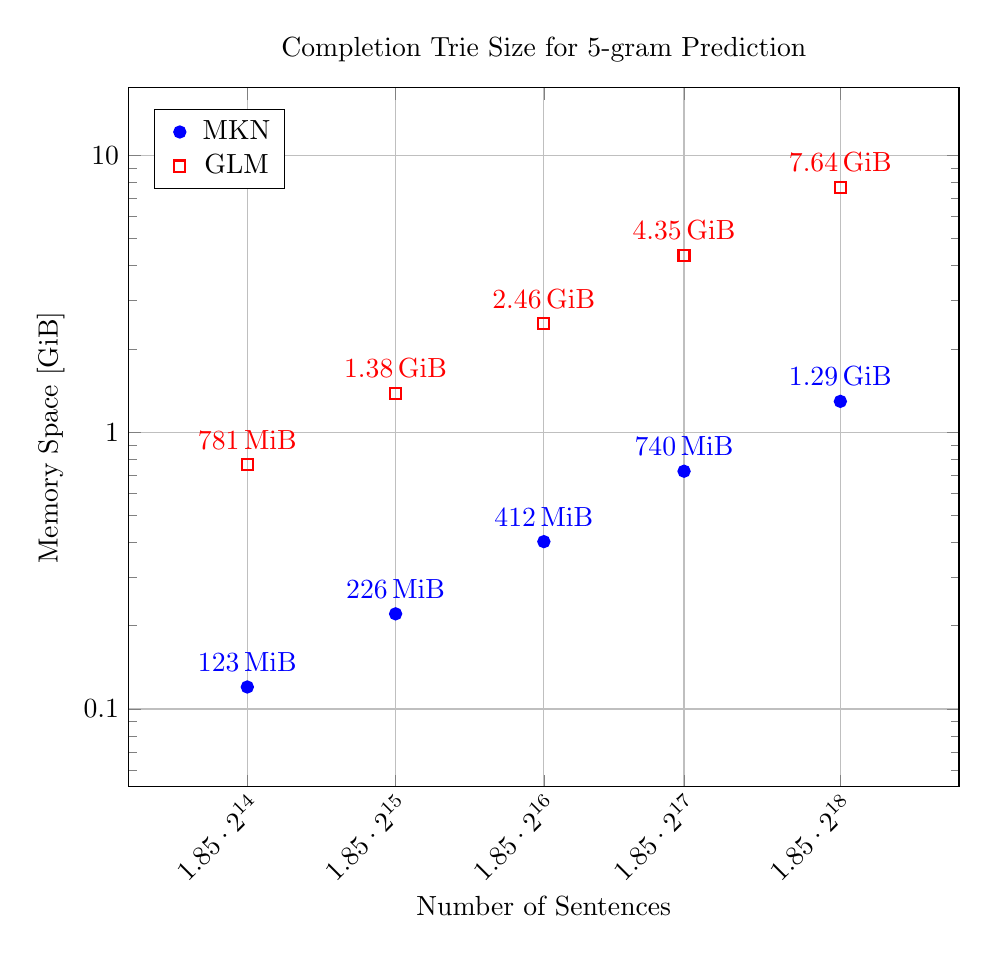
\begin{tikzpicture}[baseline]

\pgfplotscreateplotcyclelist{mkn_glm}{%
  blue,  mark size=2, mark=*,      thick,\\%
  red,   mark size=2, mark=square, thick,\\%
}

\pgfplotsset{
  legend style = {
    legend image code/.code = {
      \draw[only marks]
        plot coordinates {
          (0.3cm,0cm)
        };
      \node at (0.15cm, 0cm) {};
      \node at (0.45cm, 0cm) {};
    },
  },
}

\sisetup{exponent-base = 2}
\begin{axis}[
  title = {Completion Trie Size for $5$-gram Prediction},
  xlabel = {Number of Sentences},
  xmode = log,
  xtick       = {        30400,         60801,        121602,        234204,        486409},
  xticklabels = {\num{1.85e14}, \num{1.85e15}, \num{1.85e16}, \num{1.85e17}, \num{1.85e18}},
  xticklabel style = {
    inner sep = 1pt,
    anchor = north east,
    rotate = 45,
  },
  ylabel = {Memory Space [\si{\gibi\byte}]},
  %ytick = {100, 1000, 10000},
  %yticklabels = {\num{0.1}, \num{1.0}, \num{10.0}},
  ymode = log,
  log ticks with fixed point,
  %ymin = 0,
  minor y tick num = 4,
  grid = major,
  enlargelimits = 0.2,
  cycle list name = mkn_glm,
  legend entries = {{MKN}, {GLM}},
  legend pos = north west,
  width = \textwidth,
]

% MKN
\addplot+[
  only marks,
] table [y expr = \thisrow{mb}/1024] {
  n      mb
   30400  123
   60801  226
  121602  412
  234204  740
  486409 1323
};

\node [blue, yshift = 0.5ex] at ({axis cs: 30400, 0.12}) [above] {\SI{ 123}{\mebi\byte}};
\node [blue, yshift = 0.5ex] at ({axis cs: 60801, 0.22}) [above] {\SI{ 226}{\mebi\byte}};
\node [blue, yshift = 0.5ex] at ({axis cs:121602, 0.40}) [above] {\SI{ 412}{\mebi\byte}};
\node [blue, yshift = 0.5ex] at ({axis cs:234204, 0.72}) [above] {\SI{ 740}{\mebi\byte}};
\node [blue, yshift = 0.5ex] at ({axis cs:486409, 1.29}) [above] {\SI{1.29}{\gibi\byte}};

% GLM
\addplot+[
  only marks,
] table [y expr = \thisrow{mb}/1024] {
  n      mb
   30400  781
   60801 1412
  121602 2524
  234204 4458
  486409 7821
};

\node [ red, yshift = 0.5ex] at ({axis cs: 30400, 0.76}) [above] {\SI{ 781}{\mebi\byte}};
\node [ red, yshift = 0.5ex] at ({axis cs: 60801, 1.38}) [above] {\SI{1.38}{\gibi\byte}};
\node [ red, yshift = 0.5ex] at ({axis cs:121602, 2.46}) [above] {\SI{2.46}{\gibi\byte}};
\node [ red, yshift = 0.5ex] at ({axis cs:234204, 4.35}) [above] {\SI{4.35}{\gibi\byte}};
\node [ red, yshift = 0.5ex] at ({axis cs:486409, 7.64}) [above] {\SI{7.64}{\gibi\byte}};

%\addplot [blue, domain=30400:486409, samples=100]
%  {1.7e-5*x^0.857};
%\addplot [ red, domain=30400:486409, samples=100]
%  {1.4e-4*x^0.832};

\end{axis}

\end{tikzpicture}
\end{document}

  \end{minipage}
\end{frame}

\begin{frame}[plain]
  \centering
  \begin{minipage}{0.85\textwidth}
    \centering
    \only<1>{
      \documentclass{standalone}
\usepackage[dvipsnames,svgnames,x11names]{xcolor}
\usepackage{tikz}
\usepackage{pgfplots}
\usetikzlibrary{pgfplots.statistics}
\pgfplotsset{compat = 1.12}
\usepackage[
  group-separator={,},
  exponent-product=\cdot,
]{siunitx}
\usepackage{../thesismath}
\begin{document}
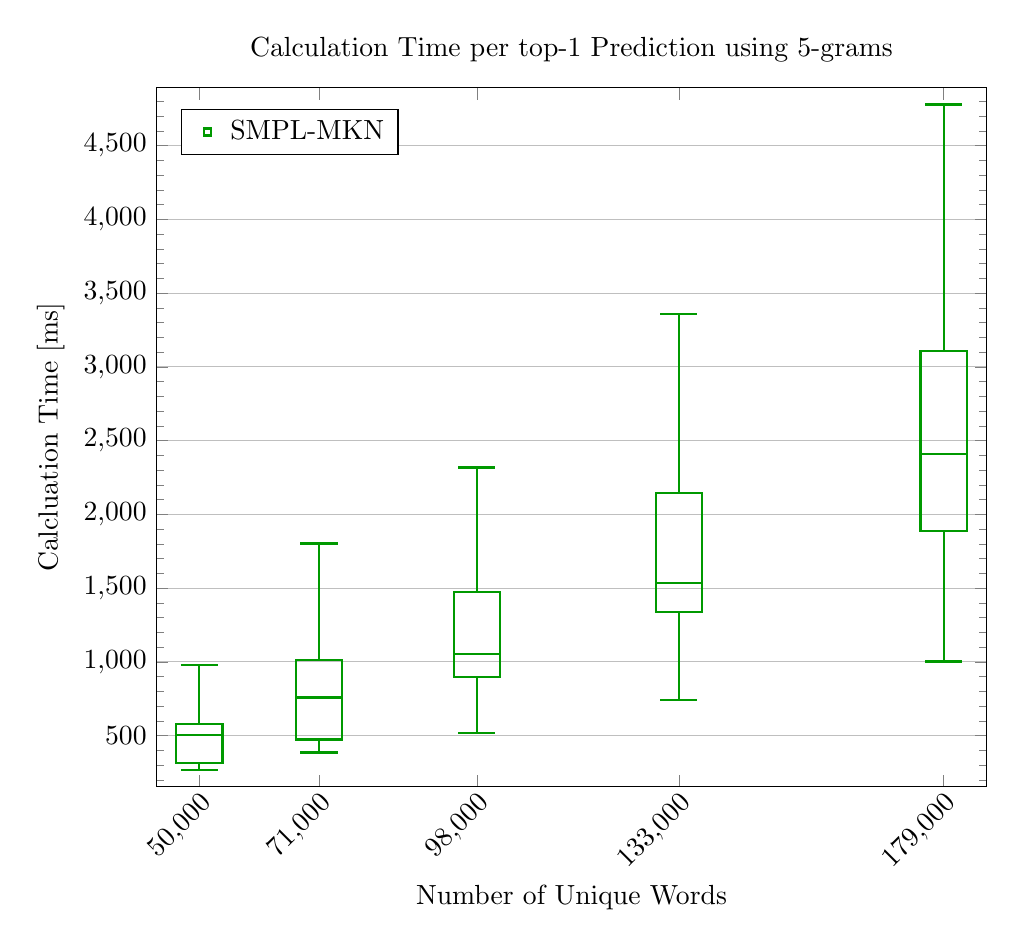
\begin{tikzpicture}[baseline]

\pgfplotscreateplotcyclelist{smpl}{%
  green!60!black,  mark size=1.25, mark=square, thick,\\%
  %blue,  mark size=1.25, mark=square,\\%
  %red,   mark size=1.25, mark=square,\\%
}

\pgfplotsset{
  legend style = {
    legend image code/.code = {
      \draw[only marks]
        plot coordinates {
          (0.3cm,0cm)
        };
      \node at (0.15cm, 0cm) {};
      \node at (0.45cm, 0cm) {};
    },
  },
  boxplot/draw/average/.code = {
    % uncomment to show dotted bars for average:
    %\draw[dashed, /pgfplots/boxplot/every average/.try]
    %  (boxplot box cs:\pgfplotsboxplotvalue{average},0)
    %  --
    %  (boxplot box cs:\pgfplotsboxplotvalue{average},1)
    %  ;
  },
}

\sisetup{exponent-base = 2}
\begin{axis}[
  title = {Calculation Time per top-$1$ Prediction using $5$-grams},
  xlabel = {Number of Unique Words},
  %xtick       = {            1,             2,             3,             4,             5},
  %xticklabels = {\num{1.85e14}, \num{1.85e15}, \num{1.85e16}, \num{1.85e17}, \num{1.85e18}},
  xtick = {50372, 70988, 98209, 133038, 178671},
  xticklabels = {\num{50000}, \num{71000}, \num{98000}, \num{133000}, \num{179000}},
  xticklabel style = {
    inner sep = 1pt,
    anchor = north east,
    rotate = 45,
  },
  ylabel = {Calcluation Time [\si{\milli\second}]},
  ymin =  265.492867,
  ymax = 4779.094746,
  scaled x ticks = false,
  scaled y ticks = false,
  minor y tick num = 4,
  ymajorgrids = true,
  boxplot/draw direction = y,
  boxplot = {
    box extend = 8000,
  },
  cycle list name = smpl,
  enlargelimits = 0.025,
  legend entries = {{SMPL-MKN}},
  legend pos = north west,
  width = \textwidth,
]

% ------------------------------------------------------------------------------

% training-5-argmaxcompare-1k-c/ngram-5-1k-SMPL-Weighted-Sum-Modified-Kneser-Ney-1
\addplot+[
  boxplot prepared = {
    %draw position = 30400,
    draw position = 50372,
    lower whisker = 265.492867,
    lower quartile = 314.299584,
    median = 502.856222,
    upper quartile = 579.864225,
    upper whisker = 976.748291,
    average = 513.082405,
  },
] table [row sep = \\, y index = 0] {
  data\\
};

% % training-5-argmaxcompare-40k-c/ngram-5-TA-Weighted-Sum-Modified-Kneser-Ney-1
% \addplot+[
%   boxplot prepared = {
%     %draw position = 30400,
%     %draw position = 50372,
%     draw position = 45372,
%     lower whisker = 0.017048,
%     lower quartile = 0.039706,
%     median = 0.058548,
%     upper quartile = 0.085849,
%     upper whisker = 0.155036,
%     average = 0.071223,
%   },
% ] table [row sep = \\, y index = 0] {
%   data\\
% };

% % training-5-argmaxcompare-40k-c/ngram-5-NRA-Weighted-Sum-Modified-Kneser-Ney-1
% \addplot+[
%   boxplot prepared = {
%     %draw position = 30400,
%     %draw position = 50372,
%     draw position = 55372,
%     lower whisker = 0.017407,
%     lower quartile = 0.042866,
%     median = 0.063964,
%     upper quartile = 0.108526,
%     upper whisker = 0.207005,
%     average = 0.367642,
%   },
% ] table [row sep = \\, y index = 0] {
%   data\\
% };

% ------------------------------------------------------------------------------

% training-4-argmaxcompare-1k-c/ngram-5-1k-SMPL-Weighted-Sum-Modified-Kneser-Ney-1
\addplot+[
  boxplot prepared = {
    %draw position = 60801,
    draw position = 70988,
    lower whisker = 385.966344,
    lower quartile = 473.753359,
    median = 758.676964,
    upper quartile = 1014.005158,
    upper whisker = 1802.043448,
    average = 800.724252,
  },
] table [row sep = \\, y index = 0] {
  data\\
};

% % training-4-argmaxcompare-40k-c/ngram-5-TA-Weighted-Sum-Modified-Kneser-Ney-1
% \addplot+[
%   boxplot prepared = {
%     %draw position = 60801,
%     %draw position = 70988,
%     draw position = 65988,
%     lower whisker = 0.019755,
%     lower quartile = 0.045715,
%     median = 0.066753,
%     upper quartile = 0.098698,
%     upper whisker = 0.178131,
%     average = 0.081448,
%   },
% ] table [row sep = \\, y index = 0] {
%   data\\
% };

% % training-4-argmaxcompare-40k-c/ngram-5-NRA-Weighted-Sum-Modified-Kneser-Ney-1
% \addplot+[
%   boxplot prepared = {
%     %draw position = 60801,
%     %draw position = 70988,
%     draw position = 75988,
%     lower whisker = 0.019593,
%     lower quartile = 0.049044,
%     median = 0.071640,
%     upper quartile = 0.117478,
%     upper whisker = 0.220049,
%     average = 0.463580,
%   },
% ] table [row sep = \\, y index = 0] {
%   data\\
% };

% ------------------------------------------------------------------------------

% training-3-argmaxcompare-1k-c/ngram-5-1k-SMPL-Weighted-Sum-Modified-Kneser-Ney-1
\addplot+[
  boxplot prepared = {
    %draw position = 121602,
    draw position = 98209,
    lower whisker = 518.403279,
    lower quartile = 898.427997,
    median = 1050.791946,
    upper quartile = 1476.127982,
    upper whisker = 2317.160040,
    average = 1156.278226,
  },
] table [row sep = \\, y index = 0] {
  data\\
};

% % training-3-argmaxcompare-40k-c/ngram-5-TA-Weighted-Sum-Modified-Kneser-Ney-1
% \addplot+[
%   boxplot prepared = {
%     %draw position = 121602,
%     %draw position = 98209,
%     draw position = 93209,
%     lower whisker = 0.020270,
%     lower quartile = 0.051889,
%     median = 0.074050,
%     upper quartile = 0.110448,
%     upper whisker = 0.198268,
%     average = 0.090352,
%   },
% ] table [row sep = \\, y index = 0] {
%   data\\
% };

% % training-3-argmaxcompare-40k-c/ngram-5-NRA-Weighted-Sum-Modified-Kneser-Ney-1
% \addplot+[
%   boxplot prepared = {
%     %draw position = 121602,
%     %draw position = 98209,
%     draw position = 103209,
%     lower whisker = 0.020295,
%     lower quartile = 0.054553,
%     median = 0.080047,
%     upper quartile = 0.132983,
%     upper whisker = 0.250549,
%     average = 0.441277,
%   },
% ] table [row sep = \\, y index = 0] {
%   data\\
% };

% ------------------------------------------------------------------------------

% training-2-argmaxcompare-1k-c/ngram-5-1k-SMPL-Weighted-Sum-Modified-Kneser-Ney-1
\addplot+[
  boxplot prepared = {
    %draw position = 2432004,
    draw position = 133038,
    lower whisker = 739.370986,
    lower quartile = 1335.713467,
    median = 1535.447582,
    upper quartile = 2146.337549,
    upper whisker = 3356.148393,
    average = 1727.968135,
  },
] table [row sep = \\, y index = 0] {
  data\\
};

% % training-2-argmaxcompare-40k-c/ngram-5-TA-Weighted-Sum-Modified-Kneser-Ney-1
% \addplot+[
%   boxplot prepared = {
%     %draw position = 2432004,
%     draw position = 133038,
%     draw position = 128038,
%     lower whisker = 0.021501,
%     lower quartile = 0.059342,
%     median = 0.084170,
%     upper quartile = 0.124255,
%     upper whisker = 0.221622,
%     average = 0.101046,
%   },
% ] table [row sep = \\, y index = 0] {
%   data\\
% };

% % training-2-argmaxcompare-40k-c/ngram-5-NRA-Weighted-Sum-Modified-Kneser-Ney-1
% \addplot+[
%   boxplot prepared = {
%     %draw position = 2432004,
%     %draw position = 133038,
%     draw position = 138038,
%     lower whisker = 0.019813,
%     lower quartile = 0.062182,
%     median = 0.092578,
%     upper quartile = 0.150630,
%     upper whisker = 0.283221,
%     average = 0.553668,
%   },
% ] table [row sep = \\, y index = 0] {
%   data\\
% };

% ------------------------------------------------------------------------------

% training-1-argmaxcompare-1k-c/ngram-5-1k-SMPL-Weighted-Sum-Modified-Kneser-Ney-1
\addplot+[
  boxplot prepared = {
    %draw position = 486409,
    draw position = 178671,
    lower whisker = 1002.784867,
    lower quartile = 1886.653179,
    median = 2408.640801,
    upper quartile = 3109.965427,
    upper whisker = 4779.094746,
    average = 2527.778769,
  },
] table [row sep = \\, y index = 0] {
  data\\
};

% % training-1-argmaxcompare-40k-c/ngram-5-TA-Weighted-Sum-Modified-Kneser-Ney-1
% \addplot+[
%   boxplot prepared = {
%     %draw position = 486409,
%     %draw position = 178671,
%     draw position = 173671,
%     lower whisker = 0.022592,
%     lower quartile = 0.066967,
%     median = 0.094754,
%     upper quartile = 0.136932,
%     upper whisker = 0.241880,
%     average = 0.111001,
%   },
% ] table [row sep = \\, y index = 0] {
%   data\\
% };

% % training-1-argmaxcompare-40k-c/ngram-5-NRA-Weighted-Sum-Modified-Kneser-Ney-1
% \addplot+[
%   boxplot prepared = {
%     %draw position = 486409,
%     %draw position = 178671,
%     draw position = 183671,
%     lower whisker = 0.023497,
%     lower quartile = 0.073006,
%     median = 0.110507,
%     upper quartile = 0.174697,
%     upper whisker = 0.327149,
%     average = 0.608050,
%   },
% ] table [row sep = \\, y index = 0] {
%   data\\
% };

% \draw [blue]
%   ({axis cs: 45372, 0.058548}) --
%   ({axis cs: 65988, 0.066753}) --
%   ({axis cs: 93209, 0.074050}) --
%   ({axis cs:133038, 0.084170}) --
%   ({axis cs:173671, 0.094754})
% ;
%
% \draw [red]
%   ({axis cs: 55372, 0.063964}) --
%   ({axis cs: 75988, 0.071640}) --
%   ({axis cs:103209, 0.080047}) --
%   ({axis cs:138038, 0.092578}) --
%   ({axis cs:183671, 0.110507})
% ;

\end{axis}

\end{tikzpicture}
\end{document}
}
    \only<2>{
      \documentclass{standalone}
\usepackage[dvipsnames,svgnames,x11names]{xcolor}
\usepackage{tikz}
\usepackage{pgfplots}
\usetikzlibrary{pgfplots.statistics}
\pgfplotsset{compat = 1.12}
\usepackage[
  group-separator={,},
  exponent-product=\cdot,
]{siunitx}
\usepackage{../thesismath}
\begin{document}
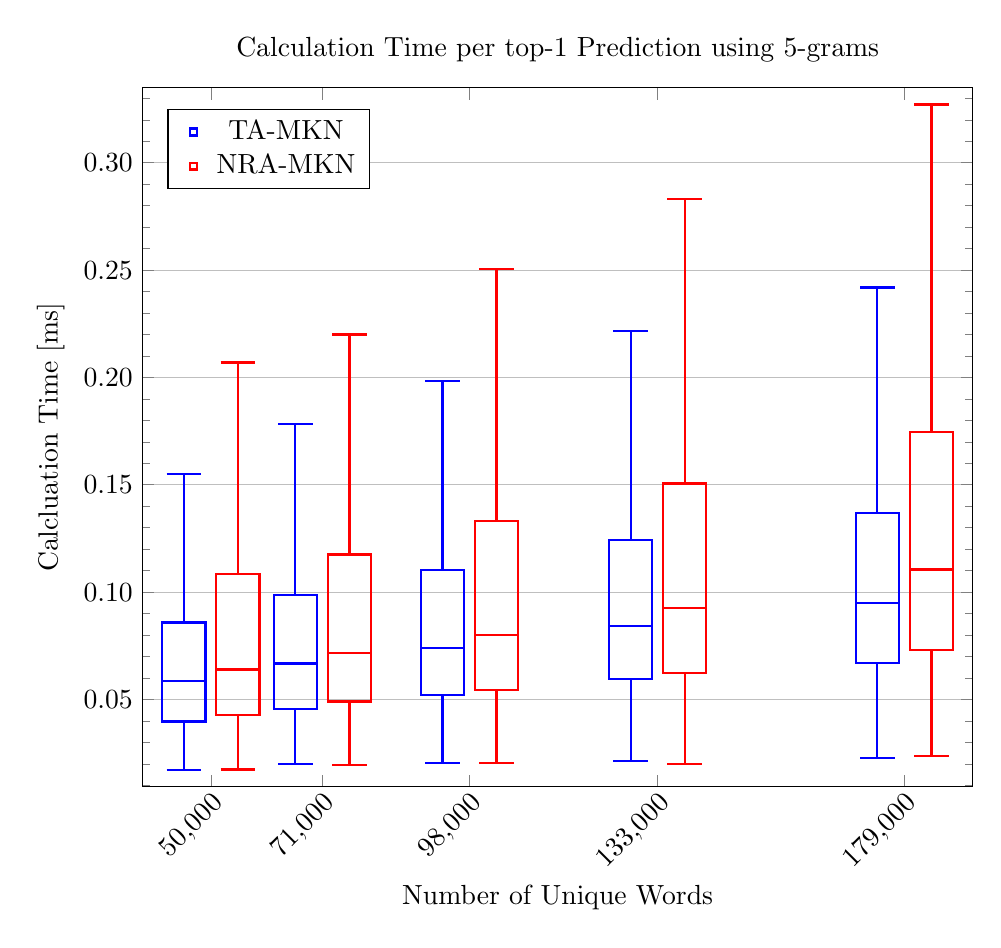
\begin{tikzpicture}[baseline]

\pgfplotscreateplotcyclelist{ta_nra}{%
  blue,  mark size=1.25, mark=square, thick,\\%
  red,   mark size=1.25, mark=square, thick,\\%
}

\pgfplotsset{
  legend style = {
    legend image code/.code = {
      \draw[only marks]
        plot coordinates {
          (0.3cm,0cm)
        };
      \node at (0.15cm, 0cm) {};
      \node at (0.45cm, 0cm) {};
    },
  },
  boxplot/draw/average/.code = {
    % uncomment to show dotted bars for average:
    %\draw[dashed, /pgfplots/boxplot/every average/.try]
    %  (boxplot box cs:\pgfplotsboxplotvalue{average},0)
    %  --
    %  (boxplot box cs:\pgfplotsboxplotvalue{average},1)
    %  ;
  },
}

\sisetup{exponent-base = 2}
\begin{axis}[
  title = {Calculation Time per top-$1$ Prediction using $5$-grams},
  xlabel = {Number of Unique Words},
  %xtick       = {            1,             2,             3,             4,             5},
  %xticklabels = {\num{1.85e14}, \num{1.85e15}, \num{1.85e16}, \num{1.85e17}, \num{1.85e18}},
  xtick = {50372, 70988, 98209, 133038, 178671},
  xticklabels = {\num{50000}, \num{71000}, \num{98000}, \num{133000}, \num{179000}},
  xticklabel style = {
    inner sep = 1pt,
    anchor = north east,
    rotate = 45,
  },
  ylabel = {Calcluation Time [\si{\milli\second}]},
  ymin = 0.01704,
  ymax = 0.32714,
  scaled x ticks = false,
  scaled y ticks = false,
  minor y tick num = 4,
  y tick label style = {
    /pgf/number format/fixed,
    /pgf/number format/fixed zerofill,
  },
  ymajorgrids = true,
  boxplot/draw direction = y,
  boxplot = {
    box extend = 8000,
  },
  cycle list name = ta_nra,
  enlargelimits = 0.025,
  legend entries = {{TA-MKN}, {NRA-MKN}},
  legend pos = north west,
  width = \textwidth,
]

% ------------------------------------------------------------------------------

% % training-5-argmaxcompare-1k-c/ngram-5-1k-SMPL-Weighted-Sum-Modified-Kneser-Ney-1
% \addplot+[
%   boxplot prepared = {
%     %draw position = 30400,
%     draw position = 50372,
%     lower whisker = 265.492867,
%     lower quartile = 314.299584,
%     median = 502.856222,
%     upper quartile = 579.864225,
%     upper whisker = 976.748291,
%     average = 513.082405,
%   },
% ] table [row sep = \\, y index = 0] {
%   data\\
% };

% training-5-argmaxcompare-40k-c/ngram-5-TA-Weighted-Sum-Modified-Kneser-Ney-1
\addplot+[
  boxplot prepared = {
    %draw position = 30400,
    %draw position = 50372,
    draw position = 45372,
    lower whisker = 0.017048,
    lower quartile = 0.039706,
    median = 0.058548,
    upper quartile = 0.085849,
    upper whisker = 0.155036,
    average = 0.071223,
  },
] table [row sep = \\, y index = 0] {
  data\\
};

% training-5-argmaxcompare-40k-c/ngram-5-NRA-Weighted-Sum-Modified-Kneser-Ney-1
\addplot+[
  boxplot prepared = {
    %draw position = 30400,
    %draw position = 50372,
    draw position = 55372,
    lower whisker = 0.017407,
    lower quartile = 0.042866,
    median = 0.063964,
    upper quartile = 0.108526,
    upper whisker = 0.207005,
    average = 0.367642,
  },
] table [row sep = \\, y index = 0] {
  data\\
};

% ------------------------------------------------------------------------------

% % training-4-argmaxcompare-1k-c/ngram-5-1k-SMPL-Weighted-Sum-Modified-Kneser-Ney-1
% \addplot+[
%   boxplot prepared = {
%     %draw position = 60801,
%     draw position = 70988,
%     lower whisker = 385.966344,
%     lower quartile = 473.753359,
%     median = 758.676964,
%     upper quartile = 1014.005158,
%     upper whisker = 1802.043448,
%     average = 800.724252,
%   },
% ] table [row sep = \\, y index = 0] {
%   data\\
% };

% training-4-argmaxcompare-40k-c/ngram-5-TA-Weighted-Sum-Modified-Kneser-Ney-1
\addplot+[
  boxplot prepared = {
    %draw position = 60801,
    %draw position = 70988,
    draw position = 65988,
    lower whisker = 0.019755,
    lower quartile = 0.045715,
    median = 0.066753,
    upper quartile = 0.098698,
    upper whisker = 0.178131,
    average = 0.081448,
  },
] table [row sep = \\, y index = 0] {
  data\\
};

% training-4-argmaxcompare-40k-c/ngram-5-NRA-Weighted-Sum-Modified-Kneser-Ney-1
\addplot+[
  boxplot prepared = {
    %draw position = 60801,
    %draw position = 70988,
    draw position = 75988,
    lower whisker = 0.019593,
    lower quartile = 0.049044,
    median = 0.071640,
    upper quartile = 0.117478,
    upper whisker = 0.220049,
    average = 0.463580,
  },
] table [row sep = \\, y index = 0] {
  data\\
};

% ------------------------------------------------------------------------------

% % training-3-argmaxcompare-1k-c/ngram-5-1k-SMPL-Weighted-Sum-Modified-Kneser-Ney-1
% \addplot+[
%   boxplot prepared = {
%     %draw position = 121602,
%     draw position = 98209,
%     lower whisker = 518.403279,
%     lower quartile = 898.427997,
%     median = 1050.791946,
%     upper quartile = 1476.127982,
%     upper whisker = 2317.160040,
%     average = 1156.278226,
%   },
% ] table [row sep = \\, y index = 0] {
%   data\\
% };

% training-3-argmaxcompare-40k-c/ngram-5-TA-Weighted-Sum-Modified-Kneser-Ney-1
\addplot+[
  boxplot prepared = {
    %draw position = 121602,
    %draw position = 98209,
    draw position = 93209,
    lower whisker = 0.020270,
    lower quartile = 0.051889,
    median = 0.074050,
    upper quartile = 0.110448,
    upper whisker = 0.198268,
    average = 0.090352,
  },
] table [row sep = \\, y index = 0] {
  data\\
};

% training-3-argmaxcompare-40k-c/ngram-5-NRA-Weighted-Sum-Modified-Kneser-Ney-1
\addplot+[
  boxplot prepared = {
    %draw position = 121602,
    %draw position = 98209,
    draw position = 103209,
    lower whisker = 0.020295,
    lower quartile = 0.054553,
    median = 0.080047,
    upper quartile = 0.132983,
    upper whisker = 0.250549,
    average = 0.441277,
  },
] table [row sep = \\, y index = 0] {
  data\\
};

% ------------------------------------------------------------------------------

% % training-2-argmaxcompare-1k-c/ngram-5-1k-SMPL-Weighted-Sum-Modified-Kneser-Ney-1
% \addplot+[
%   boxplot prepared = {
%     %draw position = 2432004,
%     draw position = 133038,
%     lower whisker = 739.370986,
%     lower quartile = 1335.713467,
%     median = 1535.447582,
%     upper quartile = 2146.337549,
%     upper whisker = 3356.148393,
%     average = 1727.968135,
%   },
% ] table [row sep = \\, y index = 0] {
%   data\\
% };

% training-2-argmaxcompare-40k-c/ngram-5-TA-Weighted-Sum-Modified-Kneser-Ney-1
\addplot+[
  boxplot prepared = {
    %draw position = 2432004,
    draw position = 133038,
    draw position = 128038,
    lower whisker = 0.021501,
    lower quartile = 0.059342,
    median = 0.084170,
    upper quartile = 0.124255,
    upper whisker = 0.221622,
    average = 0.101046,
  },
] table [row sep = \\, y index = 0] {
  data\\
};

% training-2-argmaxcompare-40k-c/ngram-5-NRA-Weighted-Sum-Modified-Kneser-Ney-1
\addplot+[
  boxplot prepared = {
    %draw position = 2432004,
    %draw position = 133038,
    draw position = 138038,
    lower whisker = 0.019813,
    lower quartile = 0.062182,
    median = 0.092578,
    upper quartile = 0.150630,
    upper whisker = 0.283221,
    average = 0.553668,
  },
] table [row sep = \\, y index = 0] {
  data\\
};

% ------------------------------------------------------------------------------

% % training-1-argmaxcompare-1k-c/ngram-5-1k-SMPL-Weighted-Sum-Modified-Kneser-Ney-1
% \addplot+[
%   boxplot prepared = {
%     %draw position = 486409,
%     draw position = 178671,
%     lower whisker = 1002.784867,
%     lower quartile = 1886.653179,
%     median = 2408.640801,
%     upper quartile = 3109.965427,
%     upper whisker = 4779.094746,
%     average = 2527.778769,
%   },
% ] table [row sep = \\, y index = 0] {
%   data\\
% };

% training-1-argmaxcompare-40k-c/ngram-5-TA-Weighted-Sum-Modified-Kneser-Ney-1
\addplot+[
  boxplot prepared = {
    %draw position = 486409,
    %draw position = 178671,
    draw position = 173671,
    lower whisker = 0.022592,
    lower quartile = 0.066967,
    median = 0.094754,
    upper quartile = 0.136932,
    upper whisker = 0.241880,
    average = 0.111001,
  },
] table [row sep = \\, y index = 0] {
  data\\
};

% training-1-argmaxcompare-40k-c/ngram-5-NRA-Weighted-Sum-Modified-Kneser-Ney-1
\addplot+[
  boxplot prepared = {
    %draw position = 486409,
    %draw position = 178671,
    draw position = 183671,
    lower whisker = 0.023497,
    lower quartile = 0.073006,
    median = 0.110507,
    upper quartile = 0.174697,
    upper whisker = 0.327149,
    average = 0.608050,
  },
] table [row sep = \\, y index = 0] {
  data\\
};

% \draw [blue]
%   ({axis cs: 45372, 0.058548}) --
%   ({axis cs: 65988, 0.066753}) --
%   ({axis cs: 93209, 0.074050}) --
%   ({axis cs:133038, 0.084170}) --
%   ({axis cs:173671, 0.094754})
% ;
%
% \draw [red]
%   ({axis cs: 55372, 0.063964}) --
%   ({axis cs: 75988, 0.071640}) --
%   ({axis cs:103209, 0.080047}) --
%   ({axis cs:138038, 0.092578}) --
%   ({axis cs:183671, 0.110507})
% ;

\end{axis}

\end{tikzpicture}
\end{document}
}
  \end{minipage}
\end{frame}

\begin{frame}[plain]
  \centering
  \begin{minipage}{0.85\textwidth}
    \centering
    \documentclass{standalone}
\usepackage[dvipsnames,svgnames,x11names]{xcolor}
\usepackage{tikz}
\usetikzlibrary{patterns}
\usepackage{pgfplots}
\pgfplotsset{compat = 1.12}
\usepackage{../thesismath}
\begin{document}
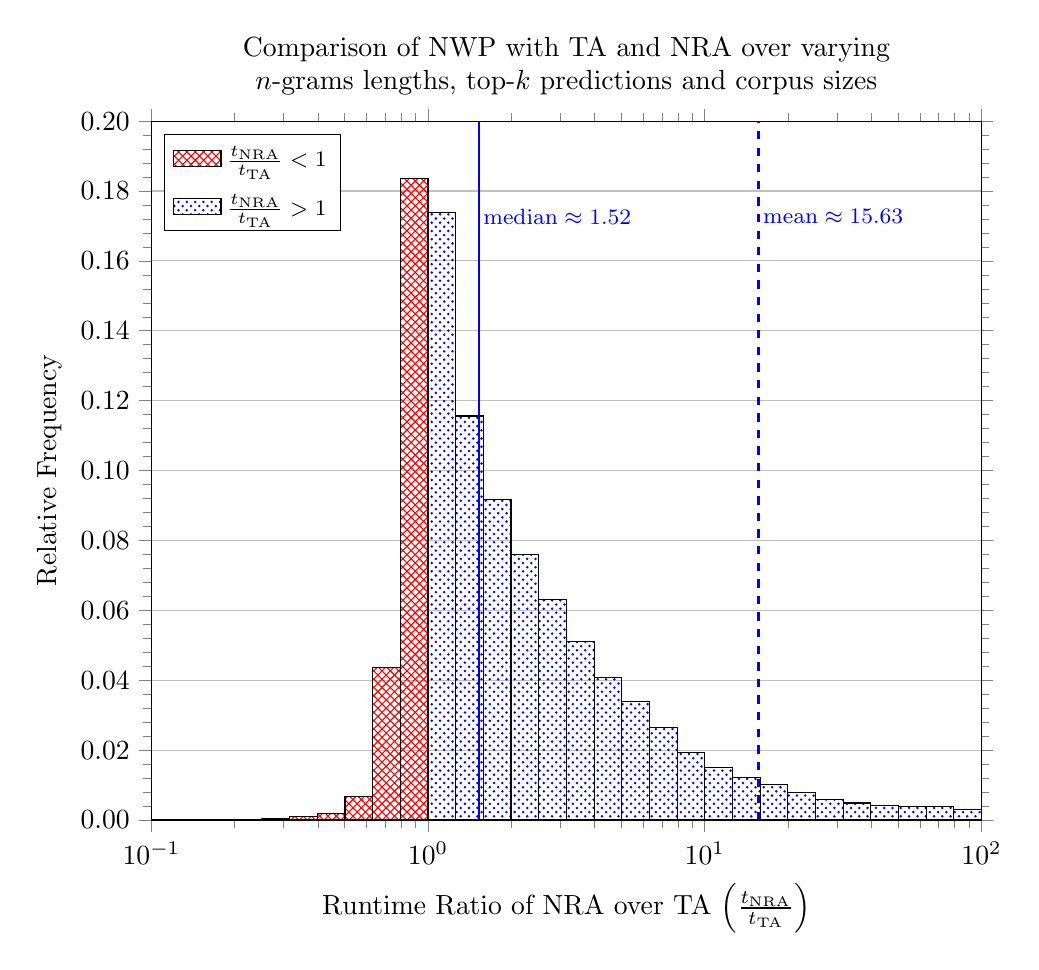
\begin{tikzpicture}[baseline]

\begin{axis}[
  align = center,
  title = {Comparison of NWP with TA and NRA over varying\\$n$-grams lengths, top-$k$ predictions and corpus sizes},
  xlabel = {Runtime Ratio of NRA over TA $\left(\frac{t_\text{NRA}}{t_\text{TA}}\right)$},
  xmode = log,
  xmin = 0.1,
  xmax = 100,
  ylabel = {Relative Frequency},
  ymin = 0,
  ymax = 0.2,
  xtick align = outside,
  ytick align = outside,
  y tick label style = {
    /pgf/number format/fixed,
    /pgf/number format/fixed zerofill,
  },
  minor y tick num = 4,
  ymajorgrids = true,
  legend entries = {{\footnotesize$\frac{t_\text{NRA}}{t_\text{TA}} < 1$},
                    {\footnotesize$\frac{t_\text{NRA}}{t_\text{TA}} > 1$}},
  legend pos = north west,
  legend style = {
    row sep = 1ex,
    xshift = -0.15cm,
    yshift =  0.1cm,
  },
  area legend,
  width = \textwidth,
]

\addplot[
  draw = black,
  pattern = crosshatch,
  pattern color = red,
  ybar interval
] plot coordinates {
  (  0.1       , 2.253787e-05)
  (  0.12589254, 2.864983e-05)
  (  0.15848932, 6.073764e-05)
  (  0.19952623, 1.247859e-04)
  (  0.25118864, 5.331415e-04)
  (  0.31622777, 8.896727e-04)
  (  0.39810717, 1.868224e-03)
  (  0.50118723, 6.792811e-03)
  (  0.63095734, 4.363942e-02)
  (  0.79432823, 1.835270e-01)
  (  1.        , 1.835270e-01)
};
\addplot[
  draw = black,
  pattern = crosshatch dots,
  pattern color = blue,
  ybar interval
] plot coordinates {
  (  1.        , 1.737457e-01)
  (  1.25892541, 1.155962e-01)
  (  1.58489319, 9.162572e-02)
  (  1.99526231, 7.606555e-02)
  (  2.51188643, 6.318370e-02)
  (  3.16227766, 5.119852e-02)
  (  3.98107171, 4.067219e-02)
  (  5.01187234, 3.396100e-02)
  (  6.30957344, 2.651421e-02)
  (  7.94328235, 1.929865e-02)
  ( 10.        , 1.498042e-02)
  ( 12.58925412, 1.207253e-02)
  ( 15.84893192, 1.025524e-02)
  ( 19.95262315, 7.834646e-03)
  ( 25.11886432, 5.825720e-03)
  ( 31.6227766 , 4.877347e-03)
  ( 39.81071706, 4.035679e-03)
  ( 50.11872336, 3.899051e-03)
  ( 63.09573445, 3.808390e-03)
  ( 79.43282347, 3.062603e-03)
  (100.        , 3.062603e-03)
};

\draw [thick, blue]
  ({axis cs:1.52357428016,0}|-{rel axis cs:0,0}) -- ({axis cs:1.52357428016,0}|-{rel axis cs:0,1})
  node [right, xshift = -0.2em, yshift = -0.1\textwidth] {\footnotesize$\text{median} \approx 1.52$};
\draw [thick, blue, dashed]
  ({axis cs:15.6303903973,0}|-{rel axis cs:0,0}) -- ({axis cs:15.6303903973,0}|-{rel axis cs:0,1})
  node [right, xshift = -0.2em, yshift = -0.1\textwidth] {\footnotesize$\text{mean} \approx 15.63$};

\end{axis}

\end{tikzpicture}
\end{document}

  \end{minipage}
\end{frame}


% % ==============================================================================
% \section{Evaluation}
% \subsection{}

% ==============================================================================
\section*{Conclusion}
\subsection{}
\begin{frame}
  \frametitle{Conclusion}
  \begin{itemize}
    \large
    \item Weighted Sum representation for probabilities
      \begin{itemize}
        \vspace{0.2cm}
        \item Calculation equally fast for MKN, double as fast for GLM
        \vspace{0.2cm}
        \item Speeds up word prediction by 50\% (MKN) to 70\% (GLM)
      \end{itemize}

    \vspace{0.6cm}
    \item Top-$k$ Joining
      \begin{itemize}
        \vspace{0.2cm}
        \item Speeds up word prediction by multiple orders of magnitude
        \vspace{-0.2cm}
        \item Threshold~Algorithm preferable to No~Random~Access~Algorithm
      \end{itemize}
  \end{itemize}
\end{frame}

\begin{frame}[plain]
  \frametitle{Thanks for your Attention!}

  \begin{center}
    {http://}{\Huge141.26.208.6}{/}
  \end{center}
\end{frame}


% ==============================================================================
\appendix
\section{Experimental Setup}
\subsection{}

\begin{frame}
  \frametitle{Evaluation Corpus}

  \large
  Open American National Corpus {\small\parencite{OANC}}
  \begin{itemize}
    \item open collection of American English
    \item historical and contemporary
    \item written text of all genres
    \item around 600.000 sentences / 14.000.000 words
  \end{itemize}
\end{frame}

\begin{frame}
  \frametitle{Experimental Setup}

  \begin{center}
    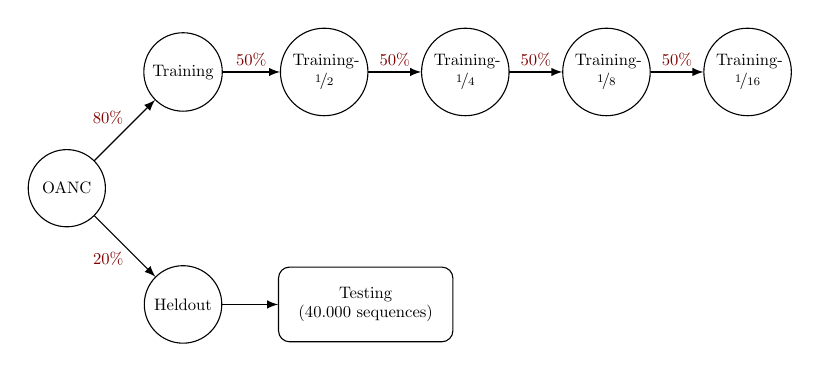
\begin{tikzpicture}
      \tikzset{
        every node/.style = {scale = 0.6},
        state/.style  = {draw, circle, align = center, text centered, text width = 3.8em},
        order/.style  = {align = center, text centered, text width = 3.8em, text = Maroon},
      }

      \begin{scope}[node distance = 7em]
        \onslide<1->{
          \node [state] (oanc)                      {OANC};
          \node         (below)    [right of=oanc]  {};
          \node [state] (training) [above of=below]  {Training};
          \node [state] (heldout)  [below of=below] {Heldout};
        }
      \end{scope}

      \begin{scope}[node distance = 8.5em]
        \onslide<3->{python api, a browser and a whole lot more.

    PermalinkSpeichernmeldenSchenke Goldantworten

[–]Schrockwell 8 Punkte 6 Stunden zuvor

But then you need 14 monitors, and 14 keyboards, and 14 more power plugs for the monitors, and 14 pairs of speakers of their mods have any sound. Laptops are all-in-one, and much easier to store after the fact.

    PermalinkSpeichernÜbergeordnetmeldenSchenke Goldantworten

[–]koffiezet 4 Punkte 4 Stunden zuvor

A lot of monitors have speakers built-in, and you'd need more stuff:

    raspberry pi's
    sd cards
    USB power supplies
    keyboards
    mice
    monitors
          \node [state] (training2) [right of=training]  {Training-\nicefrac{1}{2}};
          \node [state] (training3) [right of=training2] {Training-\nicefrac{1}{4}};
          \node [state] (training4) [right of=training3] {Training-\nicefrac{1}{8}};
          \node [state] (training5) [right of=training4] {Training-\nicefrac{1}{16}};
        }
      \end{scope}

      \begin{scope}[node distance = 11em]
        \onslide<2->{
          \node [align=center, draw, rounded corners, minimum width = 10.5em, minimum height = 4.5em]
            (testing) [right of=heldout] {Testing\\(40.000 sequences)};
        }
      \end{scope}

      \onslide<1->{
        \path[->, >=latex]
          (oanc) edge node [above, order, xshift=-1em] {80\%} (training)
          (oanc) edge node [below, order, xshift=-1em] {20\%} (heldout);
      }

      \onslide<3->{
        \path[->, >=latex]
          (training)  edge node [above, order] {50\%} (training2)
          (training2) edge node [above, order] {50\%} (training3)
          (training3) edge node [above, order] {50\%} (training4)
          (training4) edge node [above, order] {50\%} (training5);
      }

      \onslide<2->{
        \path[->, >=latex]
          (heldout) edge (testing);
      }
    \end{tikzpicture}
  \end{center}
\end{frame}


% ==============================================================================
\section{Top-k Join Examples}
\subsection{}

\begin{frame}
  \frametitle{Top-k joins combined with Weighted Sums}

  \vspace{-0.2cm}
  \onslide<2->{
    \normalsize
    \begin{equation*}
      \textstyle{\Prob{w}{h} = \sum_{i = 1}^{N} \SumWeight_i^h \; \SumArg_i^h(w)}
    \end{equation*}}

  \vspace{-0.5cm}
  \large
  \begin{itemize}
    \item<3-> Weights $\SumWeight^h_i$ can be precomputed
    \vspace{0.2cm}
    \item<4-> Sorted lists can store terms $\SumArg_i^h(w)$
  \end{itemize}

  \onslide<4->{
    \begin{center}
      \small
      \tabulinesep=1.5mm
      \begin{tabu}{ l r | l r | l r }
        \tabucline[1pt]-
        \multicolumn{2}{ c }{$\EmptyNGram$} &
        \multicolumn{2}{ c }{love} &
        \multicolumn{2}{ c }{I love} \\
        \tabucline[1pt]-

        ~the & 50~~&
        ~~\alert<6>{you} & \alert<6>{30}~~&
        ~~\alert<6>{you} & \alert<6>{25}~ \\

        ~a   & 40~~&
        ~~the & 20~~&
        ~~a   &  5~ \\

        ~\alert<6>{you} & \alert<6>{35}~~&
        ~~a   & 10~~&
        ~~the &  3~ \\
      \end{tabu}
    \end{center}}

  \large
  \begin{itemize}
    \item<5-> In examples we will assume $\SumWeight^h_1, \: \ldots, \: \SumWeight^h_N = 1$\\
      {\small(not possible in practice!)}
    \vspace{0.2cm}
    \item<6-> \alert<6>{$\Prob{\text{you}}{\text{I love}} = 35 + 30 + 25 = 95$}
  \end{itemize}
\end{frame}

\begin{frame}
  \frametitle{Threshold Algorithm}

  \begin{columns}[T]
    \begin{column}{.4\textwidth}
      \begin{enumerate}
        \item<3-> \alert< 8,12,16,18,22>{\emph{Sorted Access} to lists in any order (e.g.~round~robin)}
        \vspace{0.1cm}
        \item<4-> \alert< 9,13,19>{For new words, \emph{Random Access} to to all other lists}
        \vspace{0.1cm}
        \item<5-> \alert<11,15,17,21,23>{Compute \emph{threshold} of highest possible unseen probability}
        \vspace{0.1cm}
        \item<6-> \alert<24>{Terminate when $k$ probabilities greater threshold have been found}
      \end{enumerate}
    \end{column}
    \begin{column}{.6\textwidth}
      \onslide<1->{
        \begin{equation*}
          \textstyle{\Argmax{w \in \Vocab}\ProbMKN{w}{\text{I love}}}
        \end{equation*}}
      \vspace{-0.25cm}
      \onslide<2->{
        \tabulinesep=2mm
        \begin{tabu}{ l r | l r | l r }
          \tabucline[1pt]-
          \multicolumn{2}{ c }{$\EmptyNGram$} &
          \multicolumn{2}{ c }{love} &
          \multicolumn{2}{ c }{I love} \\
          \tabucline[1pt]-

          \tikzmark{tar1c1s} ~\action< 8->{the} & \action< 8->{50}~~\tikzmark{tar1c1e}&
          \tikzmark{tar1c2s}~~\action<12->{you} & \action<12->{30}~~\tikzmark{tar1c2e}&
          \tikzmark{tar1c3s}~~\action<13->{you} & \action<13->{25}~ \tikzmark{tar1c3e}\\

          \tikzmark{tar2c1s} ~\action<18->{a}   & \action<18->{40}~~\tikzmark{tar2c1e}&
          \tikzmark{tar2c2s}~~\action< 9->{the} & \action< 9->{20}~~\tikzmark{tar2c2e}&
          \tikzmark{tar2c3s}~~\action<19->{a}   & \action<19->{ 5}~ \tikzmark{tar2c3e}\\

          \tikzmark{tar3c1s} ~\action<13->{you} & \action<13->{35}~~\tikzmark{tar3c1e}&
          \tikzmark{tar3c2s}~~\action<19->{a}   & \action<19->{10}~~\tikzmark{tar3c2e}&
          \tikzmark{tar3c3s}~~\action< 9->{the} & \action< 9->{ 3}~ \tikzmark{tar3c3e}\\
        \end{tabu}}

        \vspace{-0.35cm}
        \begin{minipage}[t][3cm]{\textwidth}
          \begin{align*}
            \only< 7-10>{\alert< 7>{\Prob[\text{threshold}]}          &\alert< 7>{=        \infty  +        \infty  +        \infty} \hspace{-0.6em} &\alert< 7>{=}& \; \alert< 7>{\infty} \\}
            \only<11-14>{           \Prob[\text{threshold}]           &           = \alert<11>{50} +        \infty  +        \infty  \hspace{-0.6em} &           = & \;            \infty  \\}
            \only<15-16>{           \Prob[\text{threshold}]           &           =            50  + \alert<15>{30} +        \infty  \hspace{-0.6em} &           = & \;            \infty  \\}
            \only<17-20>{           \Prob[\text{threshold}]           &           =            50  +            30  + \alert<17>{25} \hspace{-0.6em} &           = & \; \alert<17>{   105} \\}
            \only<21-22>{           \Prob[\text{threshold}]           &           = \alert<21>{40} +            30  +            25  \hspace{-0.6em} &           = & \; \alert<21>{    95} \\}
            \only<14-  >{\alert<14>{\Prob{\text{you}}{\text{I love}}} &\alert<14>{=            35  +            30  +            25} \hspace{-0.6em} &\alert<14>{=}& \; \alert<14>{    90} \\}
            \only<23-  >{           \Prob[\text{threshold}]           &           =            40  + \alert<23>{20} +            25  \hspace{-0.6em} &           = & \; \alert<23>{    85} \\}
            \only<10-  >{\alert<10>{\Prob{\text{the}}{\text{I love}}} &\alert<10>{=            50  +            20  +             3} \hspace{-0.6em} &\alert<10>{=}& \; \alert<10>{    73} \\}
            \only<20-  >{\alert<20>{\Prob{\text{a  }}{\text{I love}}} &\alert<20>{=            40  +            10  +             5} \hspace{-0.6em} &\alert<20>{=}& \; \alert<20>{    55} \\}
            % For fixed alignment
            \onslide<0 >{           \Prob{\text{you}}{\text{I love}}  &           =            50  +            30  +            25  \hspace{-0.6em} &           = & \;               105}
          \end{align*}
        \end{minipage}

        
\begin{tikzpicture}[
          remember picture,
          overlay,
          iter/.style = {Maroon, thick},
        ]
          \draw< 8-17>[iter] ([yshift=-1.1ex]{pic cs:tar1c1s}) rectangle ([yshift=2.2ex]{pic cs:tar1c1e});
          \draw<12-21>[iter] ([yshift=-1.1ex]{pic cs:tar1c2s}) rectangle ([yshift=2.2ex]{pic cs:tar1c2e});
          \draw<16-  >[iter] ([yshift=-1.1ex]{pic cs:tar1c3s}) rectangle ([yshift=2.2ex]{pic cs:tar1c3e});
          \draw<18-  >[iter] ([yshift=-1.1ex]{pic cs:tar2c1s}) rectangle ([yshift=2.2ex]{pic cs:tar2c1e});
          \draw<22-  >[iter] ([yshift=-1.1ex]{pic cs:tar2c2s}) rectangle ([yshift=2.2ex]{pic cs:tar2c2e});
        \end{tikzpicture}
    \end{column}
  \end{columns}
\end{frame}


\begin{frame}
  \frametitle{No Random Access Algorithm}

  \large
  \begin{enumerate}
    \item<2-> \emph{Sorted Access} to lists in any order
    \vspace{0.3cm}
    \item<3-> Keep track of all seen counts
    \vspace{0.3cm}
    \item<4-> Compute \emph{upper} and \emph{lower bounds} for each probability
    \vspace{0.3cm}
    \item<5-> Terminate when $k$ lower bounds greater than all other upper bounds have been found
  \end{enumerate}
\end{frame}


% ==============================================================================
\section{References}
\subsection{}

\begin{frame}[allowframebreaks]
  \frametitle{References}

  \printbibliography[heading = none]
\end{frame}

\end{document}
